\documentclass[a4paper]{article}
\usepackage[utf8]{inputenc}
\usepackage[margin=1in]{geometry}
\usepackage{setspace}
\usepackage{amsmath}
\usepackage{amssymb}
\usepackage{graphicx}




\title{Chapter 3\\Vector Analysis}
\author{solutions by Hikari}
\date{July 2021}
\begin{document}

\maketitle

\newcommand{\V}{\mathbf}
\newcommand{\M}{\mathrm}
\newcommand{\VE}{\hat{\V{e}}}
\newcommand{\del}{\boldsymbol{\nabla}}
\newcommand{\pdv}[2]{\frac{\partial#1}{\partial#2}}
\newcommand{\ppdv}[3]{\frac{\partial^2#1}{\partial#2\partial#3}}
\newcommand{\dv}[2]{\frac{d #1}{d #2}}

\section*{3.2 Vectors in 3-D Space}

\paragraph{3.2.1}
$\V{P}\times \V{Q}=\sum_i \hat{\V{e}}_i\sum_{jk}\varepsilon_{ijk}P_j Q_k$.  $P_z=Q_z=0$, so $\varepsilon_{ijk}P_j Q_k\neq0$ only when $i=z$. So $\sum_i \hat{\V{e}}_i\sum_{jk}\varepsilon_{ijk}P_j Q_k=\hat{\V{e}}_z(P_xQ_y-P_yQ_x)\neq0$ because $\V{P}$ and $\V{Q}$ are nonparallel.

\paragraph{3.2.2}
$(\V{A}\times \V{B})\cdot(\V{A}\times \V{B})=(A_xB_y-A_yB_x)^2+(A_xB_z-A_zB_x)^2+(A_yB_z-A_zB_y)^2=A_x^2B_y^2+A_x^2B_z^2+A_y^2B_x^2+A_y^2B_z^2+A_z^2B_x^2+A_z^2B_y^2-2A_xB_xA_yB_y-2A_xB_xA_zB_z-2A_yB_yA_zB_z$. $(AB)^2-(\V{A}\cdot \V{B})^2=(A_x^2+A_y^2+A_z^2)(B_x^2+B_y^2+B_z^2)-(A_xB_x+A_yB_y+A_zB_z)^2=A_x^2B_y^2+A_x^2B_z^2+A_y^2B_x^2+A_y^2B_z^2+A_z^2B_x^2+A_z^2B_y^2-2A_xB_xA_yB_y-2A_xB_xA_zB_z-2A_yB_yA_zB_z$, so $(\V{A}\times \V{B})\cdot(\V{A}\times \V{B})=(AB)^2-(\V{A}\cdot \V{B})^2$.

\paragraph{3.2.3}
$\sin(\theta+\psi)=\frac{|\V{P}\times\V{Q}|}{|\V{P}||\V{Q}|}=|(-\sin{\theta}\cos{\psi}-\cos{\theta}\sin{\psi})\hat{e_z}|=\sin{\theta}\cos{\psi}+\cos{\theta}\sin{\psi}$.

$\cos{(\theta+\psi)}=\frac{\V{P}\cdot\V{Q}}{|\V{P}||\V{Q}|}=\cos{\theta}\cos{\psi}-\sin{\theta}\sin{\psi}$.

\paragraph{3.2.4}
(a) $\V{U}\times\V{V}=-3\hat{\V{e}}_y-3\hat{\V{e}}_z$ is perpendicular with $\V{U}$ and $\V{V}$.

(b) $\frac{\V{U}\times\V{V}}{|\V{U}\times\V{V}|}=\frac{1}{\sqrt{2}}\VE_y+\frac{1}{\sqrt{2}}\VE_z$

\paragraph{3.2.5}
All the four vectors are in the same plane, so both $\V{a}\times\V{b}$ and $\V{c}\times\V{d}$ are perpendicular to the plane, so $\V{a}\times\V{b}$ and $\V{c}\times\V{d}$ are parallel, so $(\V{a}\times\V{b})\times(\V{c}\times\V{d})=0$. 

\paragraph{3.2.6}
The area of the triangle $=\frac{1}{2}|\V{B}||\V{C}|\sin\alpha=\frac{1}{2}|\V{A}||\V{C}|\sin\beta=\frac{1}{2}|\V{A}||\V{B}|\sin\gamma$. Devided by $|\V{A}||\V{B}||\V{C}|/2$, we get $\frac{\sin\alpha}{|\V{A}|}=\frac{\sin\beta}{|\V{B}|}=\frac{\sin\gamma}{|\V{C}|}$.

\paragraph{3.2.7}
$\VE_x\times\V{B}=2\VE_z-4\VE_y$, $\VE_y\times\V{B}=4\VE_x-\VE_z$, $\VE_z\times\V{B}=\VE_y-2\VE_x$ by the experiments.  $\VE_x\cdot(\VE_y\times \V{B})=\V{B}\cdot(\VE_x\times\VE_y)=\V{B}\cdot(\VE_z)=\V{B}_z=4$, $\VE_y\cdot(\VE_z\times \V{B})=\V{B}\cdot(\VE_y\times\VE_z)=\V{B}\cdot(\VE_x)=\V{B}_x=1$, $\VE_z\cdot(\VE_x\times \V{B})=\V{B}\cdot(\VE_z\times\VE_x)=\V{B}\cdot(\VE_y)=\V{B}_y=2$. So $\V{B}=\VE_x+2\VE_y+4\VE_z$.

\paragraph{3.2.8}
(a) $\V{A}\cdot\V{B}\times\V{C}=(\VE_x+\VE_y)\cdot(-\VE_x+\VE_y-\VE_z)=0$. It is true because $\V{B}$, $\V{C}$ and $\V{B}\times\V{C}$ are in the same plane, so the volume of the parallelepiped is zero.

(b) $\V{A}\times(\V{B}\times\V{C})=(\VE_x+\VE_y)\times(-\VE_x+\VE_y-\VE_z)=-\VE_x+\VE_y+2\VE_z$.

\paragraph{3.2.9}
$\V{a}\times(\V{b}\times\V{c})+\V{b}\times(\V{c}\times\V{a})+\V{c}\times(\V{a}\times\V{b})=\V{b}(\V{a}\cdot\V{c})-\V{c}(\V{a}\cdot\V{b})+\V{c}(\V{b}\cdot\V{a})-\V{a}(\V{b}\cdot\V{c})+\V{a}(\V{c}\cdot\V{b})-\V{b}(\V{c}\cdot\V{a})=0$.

\paragraph{3.2.10}
(a) $\V{A}_r=\hat{\V{r}}(\V{A}\cdot\hat{\V{r}})$ is quite obvious by the definition.

(b) $\V{A}_t=\V{A}-\V{A}_r=\V{A}(\hat{\V{r}}\cdot\hat{\V{r}})-\hat{\V{r}}(\V{A}\cdot\hat{\V{r}})=-\hat{\V{r}}\times(\hat{\V{r}}\times\V{A})$.

\paragraph{3.2.11}
If $\V{A}$, $\V{B}$, and $\V{C}$ are coplanar, then $\V{B}\times\V{C}$ is perpendicular to  $\V{B}$, $\V{C}$ and therefore perpendicular to $\V{A}$, so $\V{A}\cdot\V{B}\times\V{C}=0$. If $\V{A}\cdot\V{B}\times\V{C}=0$, then $\V{A}$ is perpendicular to $\V{B}\times\V{C}$, but $\V{B}\times\V{C}$ is perpendicular to the plane of $\V{B}$ and $\V{C}$, so $\V{A}$, $\V{B}$, and $\V{C}$ are coplanar.

\paragraph{3.2.12}
$\V{A}\cdot\V{B}\times\V{C}=-120$, $\V{A}\times(\V{B}\times\V{C})=-60\VE_x-40\VE_y+50\VE_z$, $\V{C}\times(\V{A}\times\V{B})=24\VE_x+88\VE_y-62\VE_z$, $\V{B}\times(\V{C}\times\V{A})=36\VE_x-48\VE_y+12\VE_z$.

\paragraph{3.2.13}
$(\V{A}\times\V{B})\cdot(\V{C}\times\V{D})=(\V{B}\times(\V{C}\times\V{D}))\cdot\V{A}=(\V{C}(\V{B}\cdot\V{D})-\V{D}(\V{B}\cdot\V{C}))\cdot\V{A}=(\V{A}\cdot\V{C})(\V{B}\cdot\V{D})-(\V{A}\cdot\V{D})(\V{B}\cdot\V{C})$.

\paragraph{3.2.14}
$(\V{A}\times\V{B})\times(\V{C}\times\V{D})=\V{C}(\V{A}\times\V{B}\cdot\V{D})-\V{D}(\V{A}\times\V{B}\cdot\V{C})=(\V{A}\cdot\V{B}\times\V{D})\V{C}-(\V{A}\cdot\V{B}\times\V{C})\V{D}$.

\paragraph{3.2.15}
(a) $\V{F}_2=q_2\V{v}_2\times\V{B}=\frac{\mu_0}{4\pi}\frac{q_1q_2}{r^2}\V{v}_2\times(\V{v}_1\times\hat{\V{r}})$.

(b) With $\V{v}_1$ replaced by $\V{v}_2$, $\V{v}_2$ replaced by $\V{v}_1$, $\hat{\V{r}}$ replaced by $-\hat{\V{r}}$, $\V{F}_1=-\frac{\mu_0}{4\pi}\frac{q_1q_2}{r^2}\V{v}_1\times(\V{v}_2\times\hat{\V{r}})$.

(c) $\hat{\V{r}}$ are perpendicular to $\V{v}_2,\V{v}_1$, and $\V{v}_2,\V{v}_1$ are parallel, so $\V{F}_2=-\frac{\mu_0}{4\pi}\frac{q_1q_2}{r^2}v_2v_1\hat{\V{r}}=-\V{F}_1$.

\section*{3.3 Coordinate Transformations}

\paragraph{3.3.1}
\[
\begin{pmatrix}
\cos(\varphi_1+\varphi_2)&\sin(\varphi_1+\varphi_2)\\
-\sin(\varphi_1+\varphi_2)&\cos(\varphi_1+\varphi_2)
\end{pmatrix}=
\begin{pmatrix}
\cos\varphi_2&\sin\varphi_2\\
-\sin\varphi_2&\cos\varphi_2
\end{pmatrix}
\begin{pmatrix}
\cos\varphi_1&\sin\varphi_1\\
-\sin\varphi_1&\cos\varphi_1
\end{pmatrix}
\]

\paragraph{3.3.2}
Let the three reflecting surfaces be parallel to $xy$, $xz$, $yz$ surfaces. Let the direction vector of the incident light be $(k_1,k_2,k_3)$. Then after each reflection, one of the coordinate changes sign, so the direction vector of reflected light is $(-k_1,-k_2,-k_3)$, parallel to the incident light.

\paragraph{3.3.3}
$(\V{x}')^T\V{y}'=\V{x}^T\M{S}^T\M{S}\V{y}=\V{x}^T\V{y}$ because $\M{S}$ is orthogonal.

\paragraph{3.3.4}
(a) $\det\M{S}=1$

(b) $\V{a}\cdot\V{b}=-1$, $\M{S}\V{a}\cdot\M{S}\V{b}=(0.8, 0.12, 1.16)\cdot(1.2, 0.68, -1.76)=-1$

(c) $\V{a}\times\V{b}=(-2, 1, 2)$, $\M{S}(\V{a}\times\V{b})=(-1, 2.8, 0.4)$, $\M{S}\V{a}\times\M{S}\V{b}=(-1, 2.8, 0.4)$. It is as expected because pseudovectors transform as vectors when the orthogonal transformation is not a reflection ($\det (\M{S})=-1$).

\paragraph{3.3.5}
(a) $\det (\M{S})=-1$

(b) $(\M{S}\V{a})\times(\M{S}\V{b})=(-0.4, -1.64, -2.48)$; $\M{S}(\V{a}\times\V{b})=(0.4, 1.64, 2.48)$. The sign changes.

(c) $(\M{S}\V{a}\times\M{S}\V{b})\cdot\M{S}\V{c}=-3$; $\M{S}((\V{a}\times\V{b})\cdot\V{c})=(\V{a}\times\V{b})\cdot\V{c}=3$. The sign changes.

(d) $\M{S}\V{a}\times(\M{S}\V{b}\times\M{S}\V{c})=(-0.4, -8.84, 7.12)$; $\M{S}(\V{a}\times(\V{b}\times\V{c}))=(-0.4, -8.84, 7.12)$. The sign does not change.

(e) $\V{a}\times\V{b}$ is a pseudovector, $(\V{a}\times\V{b})\cdot\V{c}$ is a pseudoscalar, $\V{a}\times(\V{b}\times\V{c})$ is a vector.

\section*{3.4 Rotations in $\mathbb{R}^3$}

\paragraph{3.4.1}
The corresponding transformation matrix is 
\[
\begin{pmatrix}
\cos\psi&\sin\psi&0\\
-\sin\psi&\cos\psi&0\\
0&0&1\\
\end{pmatrix}
\begin{pmatrix}
1&0&0\\
0&\cos\theta&\sin\theta\\
0&-\sin\theta&\cos\theta\\
\end{pmatrix}
\begin{pmatrix}
\cos\varphi&\sin\varphi&0\\
-\sin\varphi&\cos\varphi&0\\
0&0&1\\
\end{pmatrix}
\]
Make the substitution by $\cos\varphi=-\sin\alpha$, $\sin\varphi=\cos\alpha$, $\cos\theta=\cos\beta$, $\sin\theta=\sin\beta$, $\cos\psi=\sin\gamma$, $\sin\psi=-\cos\gamma$. The matrix becomes
\[
\begin{pmatrix}
\sin\gamma&-\cos\gamma&0\\
\cos\gamma&\sin\gamma&0\\
0&0&1\\
\end{pmatrix}
\begin{pmatrix}
1&0&0\\
0&\cos\beta&\sin\beta\\
0&-\sin\beta&\cos\beta\\
\end{pmatrix}
\begin{pmatrix}
-\sin\alpha&\cos\alpha&0\\
-\cos\alpha&-\sin\alpha&0\\
0&0&1\\
\end{pmatrix}
\]
\[=
\begin{pmatrix}
\sin\gamma&-\cos\gamma&0\\
\cos\gamma&\sin\gamma&0\\
0&0&1\\
\end{pmatrix}
\begin{pmatrix}
-\sin\alpha&\cos\alpha&0\\
-\cos\beta\cos\alpha&-\cos\beta\sin\alpha&\sin\beta\\
\sin\beta\cos\alpha&\sin\beta\sin\alpha&\cos\beta\\
\end{pmatrix}
\]
\[=
\begin{pmatrix}
-\sin\gamma\sin\alpha+\cos\gamma\cos\beta\cos\alpha&
\sin\gamma\cos\alpha+\cos\gamma\cos\beta\sin\alpha&
-\cos\gamma\sin\beta\\
-\cos\gamma\sin\alpha-\sin\gamma\cos\beta\cos\alpha&
\cos\gamma\cos\alpha-\sin\gamma\cos\beta\sin\alpha&
\sin\gamma\sin\beta\\
\sin\beta\cos\alpha&
\sin\beta\sin\alpha&
\cos\beta\\
\end{pmatrix}
\]
which is the same as the transformation matrix in Eq. (3.37).

\paragraph{3.4.2}
(In the original system, the North Pole is in the $x_3$-axis direction, and the middle point of Prime Meridian($0^\circ,0^\circ$) is in the $x_2$-axis direction) Rotate $\alpha=70^\circ$ around $x_3$-axis to align $x_1$-axis with $20^\circ$ west, and rotate $\beta=60^\circ$ around $x_2$-axis to align the North Pole with $30^\circ$ north, and Rotate $\gamma=-80^\circ$ around $x_3$-axis to align the $10^\circ$ west Meridian with the Meridian in new system). Calculating from Eq. (3.37), the transformation matrix is 
\[
\begin{pmatrix}
0.9551&-0.2552&-0.1504\\
0.0052&0.5221&-0.8529\\
0.2962&0.8138&0.5000\\
\end{pmatrix}
\]

\paragraph{3.4.3}
All the trigonometric function except $\cos\beta$ change sign. Substituting, we found that the rotation matrix $\M{S}$ remains unchanged.

\paragraph{3.4.4}
$\M{S}(\alpha,\beta,\gamma)=\M{S}_3(\gamma)\M{S}_2(\beta)\M{S}_1(\alpha)$. Note that $\M{S}_i^{-1}(x)=\tilde{\M{S}}_i(x)$ (orthogonality) and $\M{S}_i(x)^{-1}=\M{S}_i(-x)$ (property of rotation matrix). So 
\[\M{S}^{-1}(\alpha,\beta,\gamma)=\M{S}_1^{-1}(\alpha)\M{S}_2^{-1}(\beta)\M{S}_3^{-1}(\gamma)=\tilde{\M{S}}_1(\alpha)\tilde{\M{S}}_2(\beta)\tilde{\M{S}}_3(\gamma)=\tilde{(\M{S}_3(\gamma)\M{S}_2(\beta)\M{S}_1(\alpha))}=\tilde{\M{S}}(\alpha,\beta,\gamma)\]
\[\M{S}^{-1}(\alpha,\beta,\gamma)=\M{S}_1^{-1}(\alpha)\M{S}_2^{-1}(\beta)\M{S}_3^{-1}(\gamma)=\M{S}_1(-\alpha)\M{S}_2(-\beta)\M{S}_3(-\gamma)=\M{S}_3(-\alpha)\M{S}_2(-\beta)\M{S}_1(-\gamma)=\M{S}(-\gamma,-\beta,-\alpha)\]

\paragraph{3.4.5}
(a) Decompose $\V{r}$ into $\V{r}_{\parallel}$ parallel to $\hat{\V{n}}$ and $\V{r_{\perp}}$ perpendicular to $\hat{\V{n}}$. 
$\V{r}_{\parallel}=\hat{\V{n}}(\hat{\V{n}}\cdot\V{r})$, $\V{r_{\perp}}=\V{r}-\hat{\V{n}}(\hat{\V{n}}\cdot\V{r})$.
After rotation, $\V{r}_{\parallel}$ remains unchanged, and $\V{r_{\perp}}$ becomes $\frac{\V{r_{\perp}}}{|\V{r_{\perp}}|}\times\hat{\V{n}}(|\V{r_{\perp}}|\sin\V{\Phi})$ in the $\VE_{\V{\Phi}}$ direction and $\frac{\V{r_{\perp}}}{|\V{r_{\perp}}|}|\V{r_{\perp}}|\cos\V{\Phi}$ in the $\VE_{\V{r}_{\perp}}$ direction. So 
\[\V{r}'=\V{r}_{\parallel}+\V{r_{\perp}}\times\hat{\V{n}}\sin\V{\Phi}+\V{r_{\perp}}\cos\V{\Phi}=\hat{\V{n}}(\hat{\V{n}}\cdot\V{r})+(\V{r}-\hat{\V{n}}(\hat{\V{n}}\cdot\V{r}))\times\hat{\V{n}}\sin\V{\Phi}+(\V{r}-\hat{\V{n}}(\hat{\V{n}}\cdot\V{r}))\cos\V{\Phi}\]
\[
=\V{r}\cos\V{\Phi}+\V{r}\times\hat{\V{n}}\sin\V{\Phi}+\hat{\V{n}}(\hat{\V{n}}\cdot\V{r})(1-\cos\V{\Phi})
\]

(b) Let $\V{r}=(x,y,z)$, then 
\[
\V{r}'=
\begin{pmatrix}x'\\y'\\z'\end{pmatrix}=
\begin{pmatrix}x\cos\V{\Phi}\\y\cos\V{\Phi}\\z\cos\V{\Phi}\end{pmatrix}+
\begin{pmatrix}y\sin\V{\Phi}\\-z\sin\V{\Phi}\\0\end{pmatrix}+
\begin{pmatrix}0\\0\\z(1-\cos\V{\Phi})\end{pmatrix}=
\begin{pmatrix}x\cos\V{\Phi}+y\sin\V{\Phi}\\-z\sin\V{\Phi}+y\cos\V{\Phi}\\z\end{pmatrix}
\]
\[
\begin{pmatrix}x'\\y'\\z'\end{pmatrix}=
\begin{pmatrix}
\cos\V{\Phi}&\sin\V{\Phi}&0\\
-\sin\V{\Phi}&\cos\V{\Phi}&0\\
0&0&1
\end{pmatrix}
\begin{pmatrix}x\\y\\z\end{pmatrix}
\]
which is identical with Eq. (3.55).

(c)
$\V{r}\cdot(\V{r}\times\hat{\V{n}})=0$, $(\V{r}\times\hat{\V{n}})\cdot\hat{\V{n}}=0$ because they are perpendicular. Let $\theta$ be the angle between $\V{r}$ and $\hat{\V{n}}$, then $|\V{r}\times\hat{\V{n}}|=r\sin\theta$, $|\hat{\V{n}}\cdot\V{r}|=r\cos\theta$. \[r'^2=\V{r}'\cdot\V{r}'=r^2\cos^2\Phi+(\V{r}\times\hat{\V{n}})^2\sin^2\Phi+(\hat{\V{n}}\cdot\V{r})^2(1-\cos\Phi)^2+2(\hat{\V{n}}\cdot\V{r})^2(\cos\Phi)(1-\cos\Phi)\]
\[
=r^2\cos^2\Phi+r^2\sin^2\theta\sin^2\Phi+r^2\cos^2\theta(1-\cos\Phi)^2+2r^2\cos^2\theta(\cos\Phi)(1-\cos\Phi)
\]
\[=r^2\cos^2\Phi+r^2\sin^2\theta\sin^2\Phi+r^2\cos^2\theta(1-\cos^2\Phi)
\]
\[
=r^2\cos^2\Phi+r^2\sin^2\Phi
\]
\[
=r^2
\]

\section*{3.5 Differential Vector Operators}

\paragraph{3.5.1}
(a) $\del\V{S}=-3(x^2+y^2+z^2)^{-5/2}(x\VE_x+y\VE_y+z\VE_z)=-3(14)^{-5/2}(1\VE_x+2\VE_y+3\VE_z)$ at point $(1,2,3)$.

(b) $\del\V{S}=3\cdot14^{-5/2}\cdot14^{1/2}=\frac{3}{196}$

(c) $(\frac{-1}{\sqrt{14}},\frac{-2}{\sqrt{14}},\frac{-3}{\sqrt{14}})$

\paragraph{3.5.2}
(a) $(\pdv{f}{x},\pdv{f}{y},\pdv{f}{z})\cdot(dx,dy,dz)=df=0$ when $f(x,y,z)=constant$, so $(\pdv{f}{x},\pdv{f}{y},\pdv{f}{z})$ is perpendicular to the equipotential surfaces. $\del(x^2+y^2+z^2)=2x\VE_x+2y\VE_y+2z\VE_z=2\VE_x+2\VE_y+2\VE_z$ at point $(1,1,1)$, and its unit vector is $\frac{\VE_x+\VE_y+\VE_z}{\sqrt{3}}$.

(b) $(x-1,y-1,z-1)\cdot(1,1,1)=0$, so the tangent surface is $x+y+z=3$.

\paragraph{3.5.3}
$r_{12}=\sqrt{(x_1-x_2)^2+(y_1-y_2)^2+(z_1-z_2)^2}$, so $\del_1r_{12}=\pdv{r_{12}}{x}\VE_x+\pdv{r_{12}}{y}\VE_y+\pdv{r_{12}}{z}\VE_z=\frac{x_1-x_2}{r_{12}}\VE_x+\frac{y_1-y_2}{r_{12}}\VE_y+\frac{z_1-z_2}{r_{12}}\VE_z=\frac{\V{r_{12}}}{r_{12}}$ which is the unit vector in the direction of $\V{r_{12}}$.

\paragraph{3.5.4}
\[\V{F}=F_x\VE_x+F_y\VE_y+F_z\VE_z\]
\[
d\V{F}=(\pdv{F_x}{x}dx+\pdv{F_x}{y}dy+\pdv{F_x}{z}dz+\pdv{F_x}{t}dt)\VE_x+(\pdv{F_y}{x}dx+\pdv{F_y}{y}dy+\pdv{F_y}{z}dz+\pdv{F_y}{t}dt)\VE_y+(\pdv{F_z}{x}dx+\pdv{F_z}{y}dy+\pdv{F_z}{z}dz+\pdv{F_z}{t}dt)\VE_z
\]
\[=
(dx\pdv{}{x}+dy\pdv{}{y}+dz\pdv{}{z})F_x\VE_x+(dx\pdv{}{x}+dy\pdv{}{y}+dz\pdv{}{z})F_y\VE_y+(dx\pdv{}{x}+dy\pdv{}{y}+dz\pdv{}{z})F_z\VE_z+(\pdv{F_x}{t}\VE_x+\pdv{F_y}{t}\VE_y+\pdv{F_z}{t}\VE_z)dt
\]
\[
=(dx\pdv{}{x}+dy\pdv{}{y}+dz\pdv{}{z})(F_x\VE_x+F_y\VE_y+F_z\VE_z)+\pdv{\V{F}}{t}dt
\]
\[
=(d\V{r}\cdot\del)\V{F}+\pdv{\V{F}}{t}dt
\]

\paragraph{3.5.5}
$\del(uv)=\pdv{uv}{x}\VE_x+\pdv{uv}{y}\VE_y+\pdv{uv}{z}\VE_z=(\pdv{u}{x}v+u\pdv{v}{x})\VE_x+(\pdv{u}{y}v+u\pdv{v}{y})\VE_y+(\pdv{u}{z}v+u\pdv{v}{z})\VE_z$\\
$=(\pdv{u}{x}\VE_x+\pdv{u}{y}\VE_y+\pdv{u}{z}\VE_z)v+u(\pdv{v}{x}\VE_x+\pdv{v}{y}\VE_y+\pdv{v}{z}\VE_z)=v\del u+u\del v$

\paragraph{3.5.6}
(a) $\Dot{\V{r}}=\frac{d\V{r}}{dt}=-r\omega\sin{\omega t}\,\VE_x+r\omega\cos{\omega t}\,\VE_y$, so 
\[\V{r}\times\Dot{\V{r}}=(r\cos{\omega t}\,\VE_x+r\sin{\omega t}\,\VE_t)\times(-r\omega\sin{\omega t}\,\VE_x+r\omega\cos{\omega t}\,\VE_y)=r\omega^2(\cos^2{\omega t}+\sin^2{\omega t})\VE_z=r\omega^2\VE_z\]

(b) $\Ddot{\V{r}}=-r\omega^2\cos{\omega t}\,\VE_x-r\omega^2\sin{\omega t}\,\VE_y$, so $\Ddot{\V{r}}+\omega^2\V{r}=0$.

\paragraph{3.5.7}
$\V{A'}=\M{S}\V{A}$, which means $A'_i=\sum_{j}\M{S}_{ij}A_j$. Because $\M{S}_{ij}$ is independent of $t$, so $\frac{dA'_i}{dt}=\sum_{j}\M{S}_{ij}\frac{dA_j}{dt}$, which means $\frac{d\V{A'}}{dt}=\M{S}\frac{d\V{A}}{dt}$.

\paragraph{3.5.8}
(a) $\frac{d}{dt}(\V{A}\cdot\V{B})=\frac{d}{dt}(A_xB_x+A_yB_y+A_zB_z)=\frac{dA_x}{dt}B_x+A_x\frac{dB_x}{dt}+\frac{dA_y}{dt}B_y+A_y\frac{dB_y}{dt}+\frac{dA_z}{dt}B_z+A_z\frac{dB_z}{dt}$\\
$=\frac{d\V{A}}{dt}\cdot\V{B}+\V{A}\cdot\frac{d\V{B}}{dt}$
\medskip

(b) 
\[
\frac{d}{dt}(\V{A}\times\V{B})=\frac{d}{dt}\bigg( (A_yB_z-A_zB_y)\VE_x+(A_zB_x-A_xB_z)\VE_y+(A_xB_y-A_yB_x)\VE_z \bigg)
\]
\[
=
\scriptstyle\left(\dv{A_y}{t}B_z+A_y\dv{B_z}{t}-\dv{A_z}{t}B_y-A_z\dv{B_y}{t}\right)\VE_x+\left(\dv{A_z}{t}B_x+A_z\dv{B_x}{t}-\dv{A_x}{t}B_z-A_x\dv{B_z}{t}\right)\VE_y+\left(\dv{A_x}{t}B_y+A_x\dv{B_y}{t}-\dv{A_y}{t}B_x-A_y\dv{B_x}{t}\right)\VE_z
\]
\[
=
\scriptstyle\left(\dv{A_y}{t}B_z-\dv{A_z}{t}B_y\right)\VE_x+\left(\dv{A_z}{t}B_x-\dv{A_x}{t}B_z\right)\VE_y+\left(\dv{A_x}{t}B_y-\dv{A_y}{t}B_x\right)\VE_z+
\left(A_y\dv{B_z}{t}-A_z\dv{B_y}{t}\right)\VE_x+\left(A_z\dv{B_x}{t}-A_x\dv{B_z}{t}\right)\VE_y+\left(A_x\dv{B_y}{t}-A_y\dv{B_x}{t}\right)\VE_z
\]

\[
=\dv{\V{A}}{t}\times\V{B}+\V{A}\times\dv{\V{B}}{t}
\]

\paragraph{3.5.9}
$\frac{d}{dx}a_ib_j=\frac{da_i}{dx}b_j+a_i\frac{db_j}{dx}$, so we can decompose $\del\cdot(\V{a}\times\V{b})$ into $\del_a\cdot(\V{a}\times\V{b})+\del_b\cdot(\V{a}\times\V{b})$, with $\del_a$ operating on $\V{a}$ only, and $\del_b$ operating on $\V{b}$ only. Then by the symmetry of scalar triple product, $\del_a\cdot(\V{a}\times\V{b})=\V{b}\cdot(\del_a\times\V{a})=\V{b}\cdot(\del\times\V{a})$, and $\del_b\cdot(\V{a}\times\V{b})=\V{a}\cdot(\V{b}\times\del_b)=-\V{a}\cdot(\del_b\times\V{b})=-\V{a}\cdot(\del\times\V{b})$. So $\del\cdot(\V{a}\times\V{b})=\V{b}\cdot(\del\times\V{a})-\V{a}\cdot(\del\times\V{b})$.

\paragraph{3.5.10}
$\V{L}=\V{r}\times(-i\del)=(x\VE_x+y\VE_y+z\VE_z)\times(-i\pdv{}{x}\VE_x-i\pdv{}{y}\VE_y-i\pdv{}{z}\VE_z)=\\-i\left(y\pdv{}{z}-z\pdv{}{y} \right)\VE_x-i\left(z\pdv{}{x}-x\pdv{}{z} \right)\VE_y-i\left(x\pdv{}{y}-y\pdv{}{x} \right)\VE_z$

\paragraph{3.5.11}
\[L_xL_y-L_yL_x\]
\[
=-\left(y\pdv{}{z}-z\pdv{}{y} \right)\left(z\pdv{}{x}-x\pdv{}{z} \right)+\left(z\pdv{}{x}-x\pdv{}{z} \right)\left(y\pdv{}{z}-z\pdv{}{y} \right)
\]
\[
=-\left(y\pdv{}{x}+yz\ppdv{}{z}{x}-yx\pdv{^2}{z^2}-z^2\ppdv{}{y}{x}+xz\ppdv{}{y}{z} \right)+\left(zy\ppdv{}{x}{z}-z^2\ppdv{}{x}{y}-xy\pdv{^2}{z^2}+x\pdv{}{y}+xz\ppdv{}{z}{y} \right)
\]
\[
=x\pdv{}{y}-y\pdv{}{x}=iL_z
\]

\paragraph{3.5.12}
The problem is ill-defined because the way of vector multiplication has not been specified(scalar product, cross product or tensor product). If $[\V{a},\V{b}]=0$, $[\V{a},\V{L}]=0$, $[\V{b},\V{L}]=0$ means $[a_i,b_j]=0$, $[a_i,L_j]=0$, $[b_i,L_j]=0$ for all $i,j\in\{x,y,z\}$, then $a$ and $b$, $a$ and $L$, $b$ and $L$ commute, but $L$ and $L$ do not commute ($[L_i,L_j]=iL_k$). So 
\[[\V{a}\cdot\V{L},\V{b}\cdot\V{L}]\]
\[=[a_xL_x+a_yL_y+a_zL_z,b_xL_x+b_yL_y+b_zL_z]\]
\[=\sum_{i=1}^3\sum_{j=1}^3[a_iL_i,b_jL_j]\]
\[
=\sum_{i=1}^3\sum_{j=1}^3 (a_iL_ib_jL_j-b_jL_ja_iL_i)\]
\[
=\sum_{i=1}^3\sum_{j=1}^3(a_ib_jL_iL_j-b_ja_iL_jL_i)
\]
\[=
\scriptstyle a_xb_y(L_xL_y-L_yL_x)+a_xb_z(L_xL_z-L_zL_x)+a_yb_x(L_yL_x-L_xL_y)+a_yb_z(L_yL_z-L_zL_y)+a_zb_x(L_zL_x-L_xL_z)+a_zb_y(L_zL_y-L_yL_z)
\]
\[
=a_xb_yiL_z-a_xb_ziL_y-a_yb_xiL_z+a_yb_ziL_x+a_zb_xiL_y-a_zb_yiL_x
\]
\[
=i(a_yb_z-a_zb_y)L_x+i(a_zb_x-a_xb_z)L_y+i(a_xb_y-a_yb_x)L_z
\]
\[
=i(\V{a}\times\V{b})\cdot\V{L}
\]


\paragraph{3.5.13}
A stream line of a vector field should be parallel to the vector at every point in the space. So $\frac{dy}{dx}=\frac{b_y}{b_x}=\frac{x}{-y}$, where $y=y(x)$ is a stream line. Solving  the differential equation, $xdx+ydy=0$, $\frac{x^2}{2}+\frac{y^2}{2}=k'$, $x^2+y^2=k$, which is a circle. The direction of the stream line at $(1,1)$ is $-\VE_x+\VE_y$, which is counterclockwise relative $(0,0)$, the center of the circle. 

\section*{3.6 Differential Vector Operators: Further Properties}

\paragraph{3.6.1}
By the identity in Exercise 3.5.9, $\del\cdot(\V{u}\times\V{v})=\V{v}\cdot(\del\times\V{u})-\V{u}\cdot(\del\times\V{v})=0$ because $\del\times\V{u}=0$ and $\del\times\V{v}=0$ (irrotational).

\paragraph{3.6.2}
$\del\cdot(\V{A}\times\V{r})=\V{r}\cdot(\del\times\V{A})-\V{A}\cdot(\del\times\V{r})=0$ because both $\V{A}$ and the position vector $\V{r}=x\VE_x+y\VE_y+z\VE_z$ are irrotational, so their curl vanish.

\paragraph{3.6.3}
The linear velocity $\V{v}=\boldsymbol{\omega}\times\V{r}$, so $\del\cdot\V{v}=\del\cdot(\boldsymbol{\omega}\times\V{r})=\V{r}\cdot(\del\times\boldsymbol{\omega})-\boldsymbol{\omega}\cdot(\del\times\V{r})=0$ because the curl of constant vector $\boldsymbol{\omega}$ and position vector $\V{r}$ are zero. 

\paragraph{3.6.4}
$\del\times\V{V}\neq0$ but $\del\times(g\V{V})=g(\del\times\V{V})+(\del g)\times\V{V}=0$. So $\V{V}\cdot\big(g(\del\times\V{V})+(\del g)\times\V{V} \big)=g\V{V}\cdot(\del\times\V{V})+\V{V}\cdot((\del g)\times\V{V})=0$. But $\V{V}\cdot((\del g)\times\V{V})=0$ (perpendicular) and $g\neq 0$, so $\V{V}\cdot(\del\times\V{V})=0$.  

\paragraph{3.6.5}
All the terms of $\V{A}\times\V{B}$ have the form $A_iB_j\VE_k$, and $\pdv{}{x}(A_iB_j)=\pdv{A_i}{x}B_j+A_i\pdv{B_j}{x}$. So we can separate $\del\times(\V{A}\times\V{B})$ into $\del_A\times(\V{A}\times\V{B})$ and $\del_B\times(\V{A}\times\V{B})$, with $\del_A$ acting only on $\V{A}$, and $\del_B$ acting only on $\V{B}$. Using the BAC-CAB rule, but noting that $\del_A$ must go before $\V{A}$ and after $\V{B}$, $\del_B$ go before $\V{B}$ and after $\V{A}$, we get 
\[
\del\times(\V{A}\times\V{B})=\del_A\times(\V{A}\times\V{B})+\del_B\times(\V{A}\times\V{B})
\]
\[
=(\V{B}\cdot\del_A)\V{A}-\V{B}(\del_A\cdot\V{A})+\V{A}(\del_B\cdot\V{B})-(\V{A}\cdot\del_B)\V{B}
\]
\[
=(\V{B}\cdot\del)\V{A}-\V{B}(\del\cdot\V{A})+\V{A}(\del\cdot\V{B})-(\V{A}\cdot\del)\V{B}
\]

\paragraph{3.6.6}
\[[(\V{A}\times\del)\times\V{B}]_x=A_z\pdv{B_z}{x}-A_x\pdv{B_z}{z}-A_x\pdv{B_y}{y}+A_y\pdv{B_y}{x}
\]
\[[(\V{B}\times\del)\times\V{A}]_x=B_z\pdv{A_z}{x}-B_x\pdv{A_z}{z}-B_x\pdv{A_y}{y}+B_y\pdv{A_y}{x}
\]
\[
[\V{A}(\del\cdot\V{B})]_x=A_x\pdv{B_x}{x}+A_x\pdv{B_y}{y}+A_x\pdv{B_z}{z}
\]
\[
[\V{B}(\del\cdot\V{A})]_x=B_x\pdv{A_x}{x}+B_x\pdv{A_y}{y}+B_x\pdv{A_z}{z}
\]
Summing together we get 
\[
A_x\pdv{B_x}{x}+B_x\pdv{A_x}{x}+A_y\pdv{B_y}{x}+B_y\pdv{A_y}{x}+A_z\pdv{B_z}{x}+B_z\pdv{A_z}{x}
\]
which is $\pdv{(\V{A}\cdot\V{B})}{x}=[\del(\V{A}\cdot\V{B})]_x$. The same is for $y$ and $z$ components. Therefore,

\[\del(\V{A}\cdot\V{B})=
(\V{A}\times\del)\times\V{B}+(\V{B}\times\del)\times\V{A}+\V{A}(\del\cdot\V{B})+\V{B}(\del\cdot\V{A})
\]

\paragraph{3.6.7}
To distinguish between the two $\V{A}$, let the first $\V{A}$ be $\V{A}_1$ and the second be $\V{A}_2$. Applying BAC-CAB rule,  $\V{A}_1\times(\del\times\V{A}_2)=\del_2(\V{A}_1\cdot \V{A}_2)-(\V{A}_1\cdot\del)\V{A}_2$ with $\del_2$ acting only on $\V{A}_2$. Noting that $\del(\V{A}_1\cdot \V{A}_2)=\del_1(\V{A}_1\cdot \V{A}_2)+\del_2(\V{A}_1\cdot \V{A}_2)$ and $\del_1(\V{A}_1\cdot \V{A}_2)=\del_2(\V{A}_1\cdot \V{A}_2)$, we have $\del_2(\V{A}_1\cdot \V{A}_2)=\frac{\del(\V{A}_1\cdot \V{A}_2)}{2}$, so \[\V{A}\times(\del\times\V{A})=\frac{1}{2}\del(\V{A}\cdot \V{A})-(\V{A}\cdot\del)\V{A}\]

\paragraph{3.6.8}
\[\del(\V{A}\cdot\V{B}\times\V{r})=\del(\V{r}\cdot\V{A}\times\V{B})\]\[=\del(x[\V{A}\times\V{B}]_x+y[\V{A}\times\V{B}]_y+z[\V{A}\times\V{B}]_z)\]\[=[\V{A}\times\V{B}]_x\VE_x+[\V{A}\times\V{B}]_y\VE_y+[\V{A}\times\V{B}]_z\VE_z\]\[=\V{A}\times\V{B}\]
because $\V{A}\times\V{B}$ is constant, so $\pdv{[\V{A}\times\V{B}]_j}{x_i}=0$

\paragraph{3.6.9}
\[
[\del\times(\del\times\V{V})]_x=\ppdv{V_y}{y}{x}-\pdv{^2V_x}{z^2}-\pdv{^2V_x}{z^2}+\ppdv{V_z}{z}{x}
\]
\[
[\del(\del\cdot\V{V})]_x=\pdv{^2V_x}{x^2}+\ppdv{V_y}{x}{y}+\ppdv{V_z}{x}{z}
\]
\[
-[\del\cdot\del\V{V}]_x=-\pdv{^2V_x}{x^2}-\pdv{^2V_y}{y^2}-\pdv{^2V_z}{z^2}
\]
So $[\del\times(\del\times\V{V})]_x=[\del(\del\cdot\V{V})]_x-[\del\cdot\del\V{V}]_x$, as well as the $y$ and $z$ components. Therefore
\[\del\times(\del\times\V{V})=\del(\del\cdot\V{V})-\del\cdot\del\V{V}\]

\paragraph{3.6.10}
\[
[\del\times(\varphi\del\varphi)]_x=\pdv{}{y}\left(\varphi\pdv{\varphi}{z}\right)-\pdv{}{z}\left(\varphi\pdv{\varphi}{y}\right)
\]
\[
=\pdv{\varphi}{y}\pdv{\varphi}{z}+\varphi\ppdv{\varphi}{y}{z}-\pdv{\varphi}{z}\pdv{\varphi}{y}-\varphi\ppdv{\varphi}{z}{y}=0
\]
The same is for the $y$ and $z$ components. Therefore,
$\del\times(\varphi\del\varphi)=0$

\paragraph{3.6.11}
(a) If $\V{F}=\V{G}+k$, $k$ is a constant, then $\del\times\V{F}=\del\times\V{G}$ beacuse $\pdv{k}{x_i}=0$

(b) If $\V{F}=\V{G}+\del\varphi$, then $\del\times\V{F}=\del\times\V{G}+\del\times(\del\varphi)=\del\times\V{G}$ because $\del\times(\del\varphi)=0$. 

\paragraph{3.6.12}
From Exercise 3.6.7, $\V{v}\times(\del\times\V{v})=\frac{1}{2}\del(v^2)-(\V{v}\cdot\del)\V{v}$, so \[-\del\times\big(\V{v}\times(\del\times\V{v})\big)=-\frac{1}{2}\del\times\del(v^2)+\del\times\big((\V{v}\cdot\del)\V{v} \big)=\del\times\big((\V{v}\cdot\del)\V{v} \big)\]
because $\del\times\del(v^2)=0$.

\paragraph{3.6.13}
From Exercise 3.5.9, 
\[\del\cdot\big((\del u)\times(\del v) \big)=(\del v)\cdot\big(\del\times(\del u) \big)-(\del u)\cdot\big(\del\times(\del v) \big)=0\]
because $\del\times(\del u)=0$ and $\del\times(\del v)=0$

\paragraph{3.6.14}
$\del\cdot\del\varphi=\del^2\varphi=0$, and $\del\times\del\varphi=0$ for any $\varphi$, so $\del\varphi$ is both solenoidal and irrotational.

\paragraph{3.6.15}
By Equation (3.70), $\del\times(\del\times\V{A})=\del(\del\cdot\V{A})-(\del\cdot\del)\V{A}$, so the equation becomes\\ $\del(\del\cdot\V{A})-(\del\cdot\del)\V{A}-k^2\V{A}=0$. Let $\del\cdot$ operate on both side of the equation, and note that\\ $\del\cdot\big((\del\cdot\del)\V{A} \big)=(\del\cdot\del)(\del\cdot\V{A})$ because $\pdv{}{x_i}\left(\pdv{^2A_k}{x_j^2} \right)=\pdv{^2}{x_j^2}\left(\pdv{A_k}{x_i} \right)$. So the equation becomes\\ $(\del\cdot\del)(\del\cdot\V{A})-(\del\cdot\del)(\del\cdot\V{A})-k^2(\del\cdot\V{A})=-k^2(\del\cdot\V{A})=0$, so $\del\cdot\V{A}=0$. Substituting back to the second equation, we get  $(\del\cdot\del)\V{A}+k^2\V{A}=\del^2\V{A}+k^2\V{A}=0$

\paragraph{3.6.16}
Let $\Psi=\frac{k}{2}\Phi^2$, then \[\del^2\Psi=\frac{k}{2}\left(\pdv{^2\Phi^2}{x^2}+\pdv{^2\Phi^2}{y^2}+\pdv{^2\Phi^2}{z^2} \right)\]
\[
=\frac{k}{2}\left(\pdv{}{x}\left(2\Phi\pdv{\Phi}{x}\right)+\pdv{}{y}\left(2\Phi\pdv{\Phi}{y}\right)+\pdv{}{z}\left(2\Phi\pdv{\Phi}{z}\right)   \right)
\]
\[=\frac{k}{2}\left(2\pdv{\Phi}{x}\pdv{\Phi}{x}+2\Phi\pdv{^2\Phi}{x^2}+2\pdv{\Phi}{y}\pdv{\Phi}{y}+2\Phi\pdv{^2\Phi}{y^2}+2\pdv{\Phi}{z}\pdv{\Phi}{z}+2\Phi\pdv{^2\Phi}{z^2}\right)\]
\[
=k\left(\left(\pdv{\Phi}{x}\right)^2+\left(\pdv{\Phi}{y}\right)^2+\left(\pdv{\Phi}{z}\right)^2 \right)
=k|\del\Phi|^2
\]
because $\del^2\Phi=\pdv{^2\Phi}{x^2}+\pdv{^2\Phi}{y^2}+\pdv{^2\Phi}{z^2}=0$. So $\Psi=\frac{k}{2}\Phi^2$ is a solution of the equation.

\paragraph{3.6.17}
Substituting, we get
\renewcommand{\arraystretch}{1.5}
\[
\begin{pmatrix}
\frac{1}{c}\pdv{}{t}&-i\pdv{}{z}&i\pdv{}{y}\\
i\pdv{}{z}&\frac{1}{c}\pdv{}{t}&-i\pdv{}{x}\\
-i\pdv{}{y}&i\pdv{}{x}&\frac{1}{c}\pdv{}{t}
\end{pmatrix}
\begin{pmatrix}
B_x-i\frac{E_x}{c}\\
B_y-i\frac{E_y}{c}\\
B_z-i\frac{E_z}{c}\\
\end{pmatrix}
\]
\[
=\begin{pmatrix}
\left(\frac{1}{c}\pdv{B_x}{t}-\frac{1}{c}\pdv{E_y}{z}+\frac{1}{c}\pdv{E_z}{y} \right)+i\left(-\frac{1}{c^2}\pdv{E_x}{t}-\pdv{B_y}{z}+\pdv{B_z}{y} \right)\\
\left(\frac{1}{c}\pdv{B_y}{t}-\frac{1}{c}\pdv{E_z}{x}+\frac{1}{c}\pdv{E_x}{z} \right)+i\left(-\frac{1}{c^2}\pdv{E_y}{t}-\pdv{B_z}{x}+\pdv{B_x}{z} \right)\\
\left(\frac{1}{c}\pdv{B_z}{t}-\frac{1}{c}\pdv{E_x}{y}+\frac{1}{c}\pdv{E_y}{x} \right)+i\left(-\frac{1}{c^2}\pdv{E_z}{t}-\pdv{B_x}{y}+\pdv{B_y}{x} \right)\\
\end{pmatrix}=0
\]
The real and imaginary part must to be zero, respectively. So the three equations from the real part form  $\del\times\V{E}=-\pdv{\V{B}}{t}$, and the three equations from the imaginary part form  $\del\times\V{B}=\frac{1}{c^2}\pdv{\V{E}}{t}$.

\paragraph{3.6.18}
Note that $\boldsymbol{\sigma}_i^2=\boldsymbol{1}_2$, $\boldsymbol{\sigma}_i\boldsymbol{\sigma}_j=i\boldsymbol{\sigma}_k$. So 
\[
(\boldsymbol{\sigma}\cdot\V{a})(\boldsymbol{\boldsymbol{\sigma}}\cdot\V{b})\]
\[
=(a_x\boldsymbol{\sigma}_1+a_y\boldsymbol{\sigma}_2+a_z\boldsymbol{\sigma}_3)(b_x\boldsymbol{\sigma}_1+b_y\boldsymbol{\sigma}_2+b_z\boldsymbol{\sigma}_3)
\]
\[
=(a_xb_x+a_yb_y+a_zb_z)\boldsymbol{1}_2+(a_xb_y-a_yb_x)i\boldsymbol{\sigma}_3+(a_yb_z-a_zb_y)i\boldsymbol{\sigma}_1+(a_zb_x-a_xb_z)i\boldsymbol{\sigma}_2
\]
\[
=(\V{a}\cdot\V{b})\boldsymbol{1}_2+i\boldsymbol{\sigma}\cdot(\V{a}\times\V{b})
\]

\section*{3.7 Vector Integration}

\paragraph{3.7.1}
The total vector area is 
\[
\int d\boldsymbol{\sigma}=\frac{1}{2}\V{B}\times\V{A}+\frac{1}{2}\V{C}\times\V{B}+\frac{1}{2}\V{A}\times\V{C}+\frac{1}{2}(\V{C}-\V{B})\times(\V{A}-\V{B})=0
\]

\paragraph{3.7.2}
(a) $x^2+y^2=1$, so $y=\sqrt{1-x^2}$\,; $2xdx+2ydy=0$, so $dy=-\frac{x}{y}dx=-\frac{x}{\sqrt{1-x^2}}dx$. So
\[
w=\int(-\V{F})\cdot d\V{r}\]
\[=\int\frac{y}{x^2+y^2}dx+\int\frac{-x}{x^2+y^2}dy\]
\[=\int_1^{-1}\sqrt{1-x^2}\,dx+\int_1^{-1}\frac{x^2}{\sqrt{1-x^2}}\,dx\]
\[=\int_1^{-1}\frac{1}{\sqrt{1-x^2}}\,dx\]
\[=\int_{\frac{\pi}{2}}^{-\frac{\pi}{2}}\frac{1}{\sqrt{1-\sin^2\theta}}\cos\theta\,d\theta=-\pi\]

(b) $x^2+y^2=1$, so $y=-\sqrt{1-x^2}$\,; $2xdx+2ydy=0$, so $dy=-\frac{x}{y}dx=\frac{x}{\sqrt{1-x^2}}dx$. So
\[
w=\int(-\V{F})\cdot d\V{r}\]
\[=\int\frac{y}{x^2+y^2}dx+\int\frac{-x}{x^2+y^2}dy\]
\[=-\int_1^{-1}\sqrt{1-x^2}\,dx-\int_1^{-1}\frac{x^2}{\sqrt{1-x^2}}\,dx\]
\[=\int_1^{-1}\frac{-1}{\sqrt{1-x^2}}\,dx\]
\[=\int_{\frac{\pi}{2}}^{-\frac{\pi}{2}}\frac{-1}{\sqrt{1-\sin^2\theta}}\cos\theta\,d\theta=\pi\]

\paragraph{3.7.3}
Choose the path $(1,1)\rightarrow(1,3)\rightarrow(3,3)$. Then 
\[
w=\int_1^3\V{F}(x,1)\cdot(dx\VE_x)+\int_1^3\V{F}(3,y)\cdot(dy\VE_y)
\]
\[
=\int_1^3(x-1)\,dx+\int_1^3(3+y)\,dy
\]
\[
=2+10=12
\]

\paragraph{3.7.4}
$\oint\V{r}\cdot d\V{r}=\oint(xdx+ydy+zdz)=(\frac{x^2}{2}+\frac{y^2}{2}+\frac{z^2}{2})\big|_{\V{a}}^{\V{a}}=0$ where $\V{a}$ is the starting point.

\paragraph{3.7.5}
For the surfaces parallel to $yz$ surface, \[\int\displaylimits_{S_{yz}}\V{r}\cdot d\boldsymbol{\sigma}=\int\displaylimits_{S_{yz}}(x\VE_x+y\VE_y+z\VE_z)\cdot(d\sigma\VE_x)=\int\displaylimits_{S_{yz}}(xd\sigma)=x\]
equals to $1$ at $x=1$ and $0$ at $x=0$. The same is for $y$ and $z$, so \[\frac{1}{3}\int\displaylimits_S\V{r}\cdot d\boldsymbol{\sigma}=\frac{1}{3}(1+1+1)=1\]

\section*{3.8 Integral Theorems}

\paragraph{3.8.1}
Let $\V{a}$ be a constant vector, then \[\V{a}\cdot\oint\displaylimits_{\partial V}d\boldsymbol{\sigma}=\oint\displaylimits_{\partial V}\V{a}\cdot d\boldsymbol{\sigma}=\int\displaylimits_V(\del\cdot\V{a})d\tau=0\]
Because $\V{a}$ can be in arbitrary direction, $\oint\displaylimits_{\delta V}d\boldsymbol{\sigma}$ must be zero.

\paragraph{3.8.2}
\[
\frac{1}{3}\oint\displaylimits_S \V{r}\cdot d\boldsymbol{\sigma}=\frac{1}{3}\int\displaylimits_V (\del\cdot\V{r})d\tau=\frac{1}{3}\int\displaylimits_V 3d\tau=V
\]

\paragraph{3.8.3}
\[
\oint\displaylimits_S\V{B}\cdot d\boldsymbol{\sigma}=\oint\displaylimits_S(\del\times\V{A})\cdot d\boldsymbol{\sigma}=\int\displaylimits_V\del\cdot(\del\times\V{A})d\tau=0
\]
because the divergence of a curl vanishes.

\paragraph{3.8.4}
$\del\cdot(\varphi\V{E})=(\del\varphi)\cdot\V{E}+\varphi(\del\cdot\V{E})$, so $\rho\varphi=\varepsilon_0(\del\cdot\V{E})\varphi=\varepsilon_0\del\cdot(\varphi\V{E})-\varepsilon_0(\del\varphi)\cdot\V{E}$, and
\[
\int \rho\varphi\,d\tau=\varepsilon_0\int\del\cdot(\varphi\V{E})\,d\tau-\varepsilon_0\int(\del\varphi)\cdot\V{E}\,d\tau
\]
\[
=\varepsilon_0\oint\varphi\V{E}\cdot d\boldsymbol{\sigma}+\varepsilon_0\int E^2 d\tau
\]
$\varphi$ vanishes at least as fast as $r^{-1}$, so $\V{E}=-\del\varphi$ vanishes at least as fast as $r^{-2}$, and $\varphi\V{E}$ vanishes at least as fast as $r^{-3}$. But $d\boldsymbol{\sigma}$ is in the order of $r^2$, so $\oint\varphi\V{E}\cdot d\boldsymbol{\sigma}$ vanishes at large $r$. Therefore, 
\[
\int \rho\varphi\,d\tau=\varepsilon_0\int E^2 d\tau
\]

\paragraph{3.8.5}
$\del\cdot\V{J}=0$ because it is steady-state current distribution. So $\del\cdot(x_i\V{J})=(\del x_i)\cdot\V{J}+x_i(\del\cdot\V{J})=(\del x_i)\cdot\V{J}=\VE_i\cdot\V{J}=J_i$. So 
\[
\int J_i d\tau=\int\del\cdot(x_i\V{J})d\tau
=\oint x_i\V{J}\cdot d\boldsymbol{\sigma}=0
\]
because $\V{J}$ vanishes on the surface. So 
\[
\int\V{J}d\tau=\sum\int J_i d\tau\,\VE_i=0
\]

\paragraph{3.8.6}
\[
\frac{1}{2}\oint \V{t}\cdot d\boldsymbol{\lambda}=\frac{1}{2}\int(\del\times\V{t})\cdot d\boldsymbol{\sigma}=\frac{1}{2}\int2\VE_z\cdot d\boldsymbol{\sigma}=A
\]

\paragraph{3.8.7}
(a) $\oint\V{r}\times d\V{r}=\oint(xdy-ydx)\VE_z=2A\VE_z$ from Exercise 3.8.6 .
\medskip

(b) $\V{r}=a\cos\theta\VE_x+b\sin\theta\VE_y$, so $d\V{r}=-a\sin\theta d\theta\VE_x+b\cos\theta d\theta\VE_y$, and 
\[
\oint\V{r}\times d\V{r}=\int_0^{2\pi}ab(\cos^2\theta+\sin^2\theta)d\theta=2\pi ab=2A
\]
so the area of the ellipse is $\pi ab$.

\paragraph{3.8.8}
\[
\oint\V{r}\times d\V{r}=-\oint d\V{r}\times\V{r}
\]
\[
=-\int\displaylimits_S(d\boldsymbol{\sigma}\times\del)\times\V{r}
\]
\[
=-\int\displaylimits_S\left((dxdy\VE_z)\times(\pdv{}{x}\VE_x+\pdv{}{y}\VE_y+\pdv{}{z}\VE_z)\right)\times\V{r}
\]
\[
=-\int\displaylimits_S(-dxdy\pdv{}{y}\VE_x+dxdy\pdv{}{x}\VE_y)\times(x\VE_x+y\VE_y)
\]
\[
=-\int\displaylimits_S -2dxdy=2A
\]

\paragraph{3.8.9}
\[
\oint u\del v\cdot d\boldsymbol{\lambda}+\oint v\del u\cdot d\boldsymbol{\lambda}
=\oint\del(uv)\cdot d\boldsymbol{\lambda}
=\int\del\times(\del{uv})\cdot d\boldsymbol{\sigma}=0
\]
so $\oint u\del v\cdot d\boldsymbol{\lambda}=-\oint v\del u\cdot d\boldsymbol{\lambda}$.

\paragraph{3.8.10}
$\del\times(f\V{V})=(\del f)\times\V{V}+f(\del\times\V{V})$ from Eq. 3.73 . So
\[
\oint u\del v\cdot d\boldsymbol{\lambda}=\int\displaylimits_S\del\times(u\del v)\cdot d\boldsymbol{\sigma}
\]
\[
=\int\displaylimits_S(\del u)\times(\del v)\cdot d\boldsymbol{\sigma}+\int\displaylimits_S u(\del\times(\del v))\cdot d\boldsymbol{\sigma}
\]
\[
=\int\displaylimits_S(\del u)\times(\del v)\cdot d\boldsymbol{\sigma}
\]
because $\del\times(\del v)=0$.

\paragraph{3.8.11}
Let $\V{a}$ be a constant vector, then
\[
\int\displaylimits_V\del\cdot(\V{a}\times\V{P})d\tau=\int\displaylimits_V(\del\times\V{a})\cdot\V{P} d\tau-\int\displaylimits_V\V{a}\cdot(\del\times\V{P})d\tau=-\V{a}\cdot\int\displaylimits_V\del\times\V{P}d\tau
\]
Also, 
\[
\int\displaylimits_V\del\cdot(\V{a}\times\V{P})d\tau=\oint\displaylimits_{\partial V}\V{a}\times\V{P}\cdot d\boldsymbol{\sigma}=\oint\displaylimits_{\partial V}\V{P}\times d\boldsymbol{\sigma}\cdot\V{a}=\V{a}\cdot\oint\displaylimits_{\partial V}\V{P}\times d\boldsymbol{\sigma}
\]
So $\V{a}\cdot\left(\oint\displaylimits_{\partial V}\V{P}\times d\boldsymbol{\sigma}+\int\displaylimits_V\del\times\V{P}d\tau\right)=0$. Because $\V{a}$ can be in arbitrary direction, $\oint\displaylimits_{\partial V}\V{P}\times d\boldsymbol{\sigma}+\int\displaylimits_V\del\times\V{P}d\tau$ must be zero, and therefore \[\oint\displaylimits_{\partial V}d\boldsymbol{\sigma}\times\V{P}=\int\displaylimits_V\del\times\V{P}d\tau\]

\paragraph{3.8.12}
Let $\V{a}$ be a constant vector, then
\[
\oint\displaylimits_{\partial S}(\V{a}\varphi)\cdot d\V{r}=\V{a}\cdot\oint\displaylimits_{\partial S}\varphi d\V{r}
\]
Also, 
\[
\oint\displaylimits_{\partial S}(\V{a}\varphi)\cdot d\V{r}=\int\displaylimits_S\del\times(\varphi\V{a})\cdot d\boldsymbol{\sigma}=\int\displaylimits_S(\del\varphi)\times\V{a}\cdot d\boldsymbol{\sigma}=\int\displaylimits_S d\boldsymbol{\sigma}\times(\del\varphi)\cdot\V{a}=\V{a}\cdot\int\displaylimits_S d\boldsymbol{\sigma}\times(\del\varphi)
\]
so $\V{a}\cdot\left(\int\displaylimits_S d\boldsymbol{\sigma}\times(\del\varphi)-\oint\displaylimits_{\partial S}\varphi d\V{r} \right)=0$.  Because $\V{a}$ can be in arbitrary direction, $\int\displaylimits_S d\boldsymbol{\sigma}\times(\del\varphi)-\oint\displaylimits_{\partial S}\varphi d\V{r}$ must be zero, and therefore
\[
\int\displaylimits_S d\boldsymbol{\sigma}\times(\del\varphi)= \oint\displaylimits_{\partial S}\varphi d\V{r}
\]

\paragraph{3.8.13}
Let $\V{a}$ be a constant vector, then
\[
\oint\displaylimits_{\partial S
}(\V{a}\times\V{P})\cdot d\V{r}=\oint\displaylimits_{\partial S
}(\V{P}\times d\V{r})\cdot\V{a}=\V{a}\cdot\oint\displaylimits_{\partial S
}\V{P}\times d\V{r}
\]
Because $\V{a}$ is a constant, $\del\times(\V{a}\times\V{P})=\del_P\times(\V{a}\times\V{P})$, with $\del_P$ acting only on $\V{P}$. So $\del_P$ needs to go before $\V{P}$, but can go before and after $\V{a}$. So \[\del_P\times(\V{a}\times\V{P})\cdot d\boldsymbol{\sigma}=d\boldsymbol{\sigma}\times\del_P\cdot(\V{a}\times\V{P})=(d\boldsymbol{\sigma}\times\del_P)\cdot\V{a}\times\V{P}=-\V{a}\cdot(d\boldsymbol{\sigma}\times\del_P)\times\V{P}=-\V{a}\cdot(d\boldsymbol{\sigma}\times\del)\times\V{P}\]
and
\[
\oint\displaylimits_S(\V{a}\times\V{P})\cdot d\V{r}=\int\displaylimits_S\del\times(\V{a}\times\V{P})\cdot d\boldsymbol{\sigma}=-\int\displaylimits_S\V{a}\cdot(d\boldsymbol{\sigma}\times\del)\times\V{P}=-\V{a}\cdot\int\displaylimits_S(d\boldsymbol{\sigma}\times\del)\times\V{P}
\]
so $\V{a}\cdot\left(\int\displaylimits_S(d\boldsymbol{\sigma}\times\del)\times\V{P}+\oint\displaylimits_{\partial S
}\V{P}\times d\V{r} \right)=0$. Because $\V{a}$ can be in arbitrary direction, $\int\displaylimits_S(d\boldsymbol{\sigma}\times\del)\times\V{P}+\oint\displaylimits_{\partial S
}\V{P}\times d\V{r}$ must be zero, and therefore
\[
\int\displaylimits_S(d\boldsymbol{\sigma}\times\del)\times\V{P}=\oint\displaylimits_{\partial S
}d\V{r}\times\V{P}
\]

\section*{3.9 Potential Theory}

\paragraph{3.9.1}
$\V{F}=r^{2n}\V{r}$
\medskip

(a) $\del\cdot\V{F}=(\del r^{2n})\cdot\V{r}+r^{2n}(\del\cdot\V{r})=2nr^{2n-1}\frac{\V{r}}{r}\cdot\V{r}+r^{2n}(3)=(2n+3)r^{2n}$
\medskip

(b) $\del\times\V{F}=(\del r^{2n})\times\V{r}+r^{2n}(\del\times\V{r})=2nr^{2n-1}\frac{\V{r}}{r}\times\V{r}+0=0$
\medskip

(c) $\del\times\V{F}=0$, so the scalar potential exists. $\int_a^b\V{F}\cdot d\V{r}=-\int_a^b\del\varphi\cdot d\V{r}=-\varphi\big|_a^b=\varphi(a)-\varphi(b)$. Take the path $(0,0,0)\rightarrow(x,0,0)\rightarrow(x,y,0)\rightarrow(x,y,z)$. Then
\[
\int_{(0,0,0)}^{(x,y,z)}\V{F}\cdot d\V{r}=\int_0^x x^{2n}xdx+\int_0^y(x^2+y^2)^nydy+\int_0^z(x^2+y^2+z^2)^nzdz
\]
\[
=\frac{x^{2n+2}}{2n+2}-0+\frac{(x^2+y^2)^{n+1}}{2(n+1)}-\frac{(x^2)^{n+1}}{2(n+1)}+\frac{(x^2+y^2+z^2)^{n+1}}{2(n+1)}-\frac{(x^2+y^2)^{n+1}}{2(n+1)}
\]
\[
=\frac{r^{2n+2}}{2n+2}=\varphi(0,0,0)-\varphi(x,y,z)
\]
when $n\neq-1$. Defining $\varphi(0,0,0)$ to be zero, then $\varphi(x,y,z)=-\frac{r^{2n+2}}{2n+2}$.
\medskip

(d) If $n=-1$, 
\[
\int_{(1,1,1)}^{(x,y,z)}\V{F}\cdot d\V{r}=\int_1^x \frac{1}{x}dx+\int_1^y\frac{y}{x^2+y^2}dy+\int_1^z\frac{z}{x^2+y^2+z^2}dz
\]
\[
=\ln|x|+\frac{1}{2}\ln|\frac{x^2+y^2}{x^2}|+\frac{1}{2}\ln|\frac{x^2+y^2+z^2}{x^2+y^2}|
\]
\[
=\frac{1}{2}\ln|x^2+y^2+z^2|\]
\[=\ln r=\varphi(1,1,1)-\varphi(\V{r})
\]
Defining $\varphi(1,1,1)=0$, then $\varphi(\V{r})=-\ln r$ diverges at both the origin and infinity.

\paragraph{3.9.2}
Applying Gauss law, at $r\leq a$, $\oint\V{E}\cdot d\boldsymbol{\sigma}=E4\pi r^2=\frac{Q}{\varepsilon_0}\frac{r^3}{a^3}$, so $E=\frac{Qr}{4\pi\varepsilon_0a^3}$; at $r>a$, $\oint\V{E}\cdot d\boldsymbol{\sigma}=E4\pi r^2=\frac{Q}{\varepsilon_0}$, so $E=\frac{Qr}{4\pi\varepsilon_0r^2}$. Defining the potential to be zero at $r\to\infty$, then $\int_r^\infty \V{E}\cdot d\V{r}=\varphi(r)-\varphi(\infty)=\varphi(r)$. At $r>a$, $\varphi(r)=\int_r^\infty\frac{Q}{4\pi\varepsilon_0r^2}dr=\frac{Q}{4\pi\varepsilon_0r}$; at $r\leq a$, $\varphi(r)=\int_r^a\frac{Qr}{4\pi\varepsilon_0a^3}dr+\int_a^\infty\frac{Q}{4\pi\varepsilon_0r^2}dr=\frac{Q}{4\pi\varepsilon_0a}\left(\frac{1}{2}-\frac{1}{2}\frac{r^2}{a^2} \right)+\frac{Q}{4\pi\varepsilon_0a}=\frac{Q}{4\pi\varepsilon_0a}\left(\frac{3}{2}-\frac{1}{2}\frac{r^2}{a^2} \right)$. So the electrostatic potential is 
\[
\varphi(r)=
\begin{cases}
\frac{Q}{4\pi\varepsilon_0a}\left(\frac{3}{2}-\frac{1}{2}\frac{r^2}{a^2} \right), & r\leq a\\
\frac{Q}{4\pi\varepsilon_0r}, & r>a
\end{cases}
\]

\paragraph{3.9.3}
It can be verified that $\del\times\V{F}=0$, so the potential exists. 
\[
\int_{(0,0,0)}^{(x,y,z)}\V{F}\cdot d\V{r}=\varphi(0,0,0)-\varphi(x,y,z)
\]
\[
=\frac{GMm}{R^3}\int_{(0,0,0)}^{(x,y,z)}(-xdx-ydy+2zdz)
\]
\[
=\frac{GMm}{R^3}\left(-\frac{x^2}{2}-\frac{y^2}{2}+z^2 \right)=\varphi(0,0,0)-\varphi(x,y,z)
\]
Define $\varphi(0,0,0)$ to be zero, then \[\varphi(x,y,z)=-\frac{GMm}{R^3}\left(-\frac{x^2}{2}-\frac{y^2}{2}+z^2 \right)\] 

\paragraph{3.9.4}
$\del\cdot\V{B}=\frac{\mu_0I}{2\pi}\left(\frac{2xy}{(x^2+y^2)^2}-\frac{2xy}{(x^2+y^2)^2} \right)=0$, so the vector potential exists. If $\del\times\V{A}'=\V{B}$, and let $\del\varphi=-A_x'\VE_x$, then $\V{A}=\V{A}'+\del\varphi$ is also a vector potential with zero $x$-component because  $\del\times\V{A}=\del\times\V{A}'+\del\times(\del\varphi)=\V{B}$. Let $\V{A}=A_y\VE_y+A_z\VE_z$, then 
\[
\del\times\V{A}=\left(\pdv{A_z}{y}-\pdv{A_y}{z} \right)\VE_x-\pdv{A_z}{x}\VE_y+\pdv{A_y}{x}\VE_z
\]
\[
=-\frac{\mu_0I}{2\pi}\frac{y}{x^2+y^2}\VE_x+\frac{\mu_0I}{2\pi}\frac{x}{x^2+y^2}\VE_y
\]
For the $y$-component, $-\pdv{A_z}{x}=\frac{\mu_0I}{2\pi}\frac{x}{x^2+y^2}$, so $A_z=-\frac{\mu_0I}{4\pi}\ln(x^2+y^2)+C_1(y,z)$. For the $z$-component, $\pdv{A_y}{x}=0$, so $A_y=C_2(y,z)$. Substituting into the equation of the $x$-component, we get $-\frac{\mu_0I}{2\pi}\frac{y}{x^2+y^2}+\pdv{C_1}{y}-\pdv{C_2}{z}=-\frac{\mu_0I}{2\pi}\frac{y}{x^2+y^2}$, so the equation will be satisfied if we simply choose $C_1=C_2=0$. Therefore, 
\[
\V{A}=-\frac{\mu_0I}{4\pi}\ln(x^2+y^2)\VE_z
\]
is a vector potential of $\V{B}$.

\paragraph{3.9.5}
$\del\cdot\V{B}=3\frac{1}{r^3}-3\frac{x^2+y^2+z^2}{r^5}=0$, so the vector potential exist. As in Exercise 3.9.4, we can make one component of the vector potential be zero, and we choose the $z$-component. So $\V{A}=A_x\VE_x+A_y\VE_y$, and
\[
\del\times\V{A}=-\pdv{A_y}{z}\VE_x+\pdv{A_x}{z}\VE_y+\left(\pdv{A_y}{x}-\pdv{A_x}{y} \right)\VE_z
\]
\[
=\frac{x}{r^3}\VE_x+\frac{y}{r^3}\VE_y+\frac{z}{r^3}\VE_z
\]
so
\[
-\pdv{A_y}{z}=\frac{x}{r^3}\;\xrightarrow{integrating}\;A_y=\frac{-xz}{(x^2+y^2)r}+C_1(x,y)
\]
\[
\pdv{A_x}{z}=\frac{y}{r^3}\;\xrightarrow{integrating}\;A_x=\frac{yz}{(x^2+y^2)r}+C_2(x,y)
\]
Substituted into $\pdv{A_y}{x}-\pdv{A_x}{y}=\frac{z}{r^3}$, we get
\[
\frac{z}{r^3}+\pdv{C_1}{x}-\pdv{C_2}{y}=\frac{z}{r^3}
\]
which will be satisfied if we simply choose $C_1=C_2=0$. Therefore, 
\[
\V{A}=\frac{yz}{(x^2+y^2)r}\VE_x-\frac{xz}{(x^2+y^2)r}\VE_y
\]
is a solution of $\del\times\V{A}=\V{B}$

\paragraph{3.9.6}
If $\V{B}$ is a constant vector, then
\[
\del\times\V{A}=\frac{1}{2}\del\times(\V{B}\times\V{r})\]
\[=\frac{1}{2}\del_\V{r}\times(\V{B}\times\V{r})
\]
\[
=\frac{1}{2}[\V{B}(\del_\V{r}\cdot\V{r})-(\V{B}\cdot\del_\V{r})\V{r}]
\]
\[
=\frac{1}{2}[3\V{B}-\V{B}]=\V{B}
\]
So the two equations are satisfied by any constant vector $\V{B}$.

\paragraph{3.9.7}
(a) $\del\cdot\V{B}=\del\cdot((\del u)\times(\del v))=(\del v)\cdot(\del\times(\del u))-(\del u)\cdot(\del\times(\del v))=0$ because $\del\times(\del u)=0$ and $\del\times(\del v)=0$.
\medskip

(b) 
\[
\del\times\V{A}=\frac{1}{2}\del\times(u\del v)-\frac{1}{2}\del\times(v\del u)
\]
\[
=\frac{1}{2}(\del u)\times(\del v)+\frac{1}{2}u(\del\times(\del v))-\frac{1}{2}(\del v)\times(\del u)-\frac{1}{2}v(\del\times(\del u))
\]
\[
=(\del u)\times(\del v)=\V{B}
\]

\paragraph{3.9.8}
Let $\V{A}'=\V{A}+\del\varphi$, then $\V{B}'=\del\times(\V{A}+\del\varphi)=\del\times\V{A}=\V{B}$ because $\del\times(\del\varphi)=0$, so the left side of the equation is unchanged. $\oint\V{A}'\cdot d\V{r}=\oint \V{A}\cdot d\V{r}+\oint\del\varphi\cdot d\V{r}=\oint \V{A}\cdot d\V{r}$ because $\oint\del\varphi\cdot d\V{r}=\oint d\varphi=0$, so the right side of the equation is unchanged.

\paragraph{3.9.9}
Choose point $P$ to be the origin of the coordinate system $(0,0,0)$. Let $u=\frac{1}{r}$, $v=\varphi$, and apply Green's theorem Eq. 3.85, 
\[
\int\displaylimits_V\left(\frac{1}{r}\del^2\varphi-\varphi\del^2(\frac{1}{r}) \right)d\tau=\oint\displaylimits_{\partial V}\left(\frac{1}{r}\del\varphi-\varphi\del(\frac{1}{r}) \right)\cdot d\boldsymbol{\sigma}
\]
where the volume $V$ is a sphere centered at $(0,0,0)$ with radius $r$. Because there are no charges on or within the sphere, we have $\del^2\varphi=0$, and by Eq. 3.120, $\del^2(\frac{1}{r})=-4\pi\delta(\V{r})$. So the left side of the equation equals to $\int\displaylimits_V4\pi\varphi\delta(\V{r})d\tau=4\pi\varphi(0)$. As for the right side, \[\oint\displaylimits_{\partial V}\frac{1}{r}\del\varphi\cdot d\boldsymbol{\sigma}=\frac{1}{r}\int\displaylimits_V\del\cdot(\del\varphi)d\tau=\frac{1}{r}\int\displaylimits_V\del^2\varphi d\tau=0\] \[-\oint\displaylimits_V\varphi\del(\frac{1}{r})\cdot d\boldsymbol{\sigma}=\oint\displaylimits_V\varphi\frac{1}{r^2}\hat{\V{r}}\cdot d\boldsymbol{\sigma}=\frac{\oint\displaylimits_V\varphi d\sigma}{r^2}\]
so the equation becomes $4\pi\varphi(0)=\frac{\oint\displaylimits_V\varphi d\sigma}{r^2}$, so $\varphi(0)=\frac{\oint\displaylimits_V\varphi d\sigma}{4\pi r^2}$, which means the potential at $P$ is the average of the potential over the spherical surface centered on $P$ with radius $r$.

\paragraph{3.9.10}
$\del\times\V{B}=\mu\V{J}$ and $\V{B}=\del\times\V{A}$, so $\del\times(\del\times\V{A})=\mu\V{J}$. But $\del\times(\del\times\V{A})=\del(\del\cdot\V{A})-(\del\cdot\del)\V{A}=-\del^2\V{A}$ because $\del\cdot\V{A}=0$, so $\del^2\V{A}=-\mu\V{J}$.

\paragraph{3.9.11}
From the Maxwell's equations, $\del\times\V{B}=\mu_0\V{J}+\frac{1}{c^2}\pdv{\V{E}}{t}$, so 
\[
\del\times(\del\times\V{A})
\]
\[
=\del(\del\cdot\V{A})-(\del\cdot\del)\V{A}=\mu_0\V{J}+\frac{1}{c^2}\pdv{\V{E}}{t}
\]
Using the Lorentz gauge Eq. 3.109, \[
\del(\del\cdot\V{A})=\del(-\frac{1}{c^2}\pdv{\varphi}{t})=-\frac{1}{c^2}\pdv{}{t}(\del\varphi)=\frac{1}{c^2}\pdv{}{t}(\V{E}+\pdv{\V{A}}{t})=\frac{1}{c^2}\pdv{\V{E}}{t}+\frac{1}{c^2}\pdv{^2\V{A}}{t^2}
\]
Substitute into the first equation, we get
\[
\frac{1}{c^2}\pdv{^2\V{A}}{t^2}-\del^2\V{A}=\mu_0\V{J}
\]

\paragraph{3.9.12}
As in Exercise 3.9.4, we can make one component of the vector potential be zero, so we make $\V{A}=(A_x,0,A_z)$. So
\[
\del\times\V{A}=\pdv{A_z}{y}\VE_x+\left(\pdv{A_x}{z}-\pdv{A_z}{x} \right)\VE_y-\pdv{A_x}{y}\VE_z=B_x\VE_x+B_y\VE_y+B_z\VE_z
\]
For the $x$- and $z$-components, 
\[
\pdv{A_z}{y}=B_x\;\xrightarrow{integrating}\;A_z=\int_{y_0}^yB_x(x,y,z) dy+C_1(x,y)
\]
\[
-\pdv{A_x}{y}=B_z\;\xrightarrow{integrating}\;A_x=-\int_{y_0}^yB_z(x,y,z) dy+C_2(x,y)
\]
Substitute into the equation of $y$-component, 
\[
-\pdv{}{z}\int_{y_0}^yB_zdy+\pdv{C_2}{z}-\pdv{}{x}\int_{y_0}^yB_xdy-\pdv{C_1}{x}=B_y
\]
Let $y=y_0$, and let $C_2=0$, then 
\[
-\pdv{C_1}{x}=B_y(x,y_0,z)\;\xrightarrow{integrating}\;C_1=-\int_{x_0}^xB_y(x,y_0,z) dx
\]
Therefore, 
\[
\V{A}=-\VE_x\int_{y_0}^yB_z(x,y,z) dy+\VE_z\left[\int_{y_0}^yB_x(x,y,z) dy-\int_{x_0}^xB_y(x,y_0,z) dx \right]
\]

\section*{3.10 Curvilinear Coordinates}

\paragraph{3.10.1}
(a) The surfaces of $u=constant$ are hyperbolas with $x=0$ and $y=0$ as asymptotes when viewing from the $z$-axis.  The surfaces of $v=constant$ are hyperbolas with $y=x$ and $y=-x$ as asymptotes when viewing from the $z$-axis. The surfaces of $z=constant$ are surfaces parallel to the $x$-$y$ plane.

(b) 

\begin{figure}[h]
    \centering
    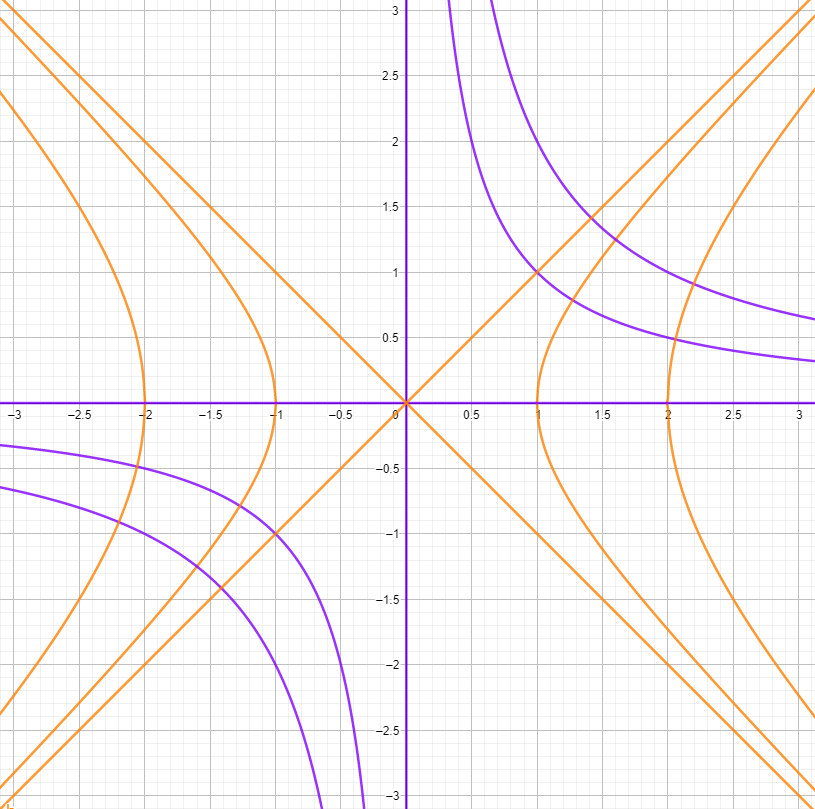
\includegraphics[width=0.5\textwidth]{B.PNG}
    \caption{The purple lines are $xy=0$, $xy=1$, $xy=2$} the orange lines are $x^2-y^2=0$, $x^2-y^2=1$, $x^2-y^2=2$.
    \label{fig:B}
\end{figure}

(c) Take the derivative of $xy=u$ we get $ydx+xdy=0$. That is, $(y,x)\cdot(dx,dy)=0$, so $(y,x)$ is a normal vector of $xy=u$ and therefore in the direction of $\VE_u$. Because $\pdv{u}{x}=y$, so $\VE_u$ should be in the direction of $(y,x)$, not $(-y,-x)$. Normalizing, we get $\VE_u=\frac{y}{\sqrt{x^2+y^2}}\VE_x+\frac{x}{\sqrt{x^2+y^2}}\VE_y$. By a similar process, from $2xdx-2ydy=0$, we get $\VE_v=\frac{x}{\sqrt{x^2+y^2}}\VE_x+\frac{-y}{\sqrt{x^2+y^2}}\VE_y$.

(d) $\VE_u\times\VE_v=\frac{-x^2-y^2}{x^2+y^2}\VE_z=-\VE_z$, so it is a left-handed system.

\paragraph{3.10.2}

\,

\begin{figure}[h]
    \centering
    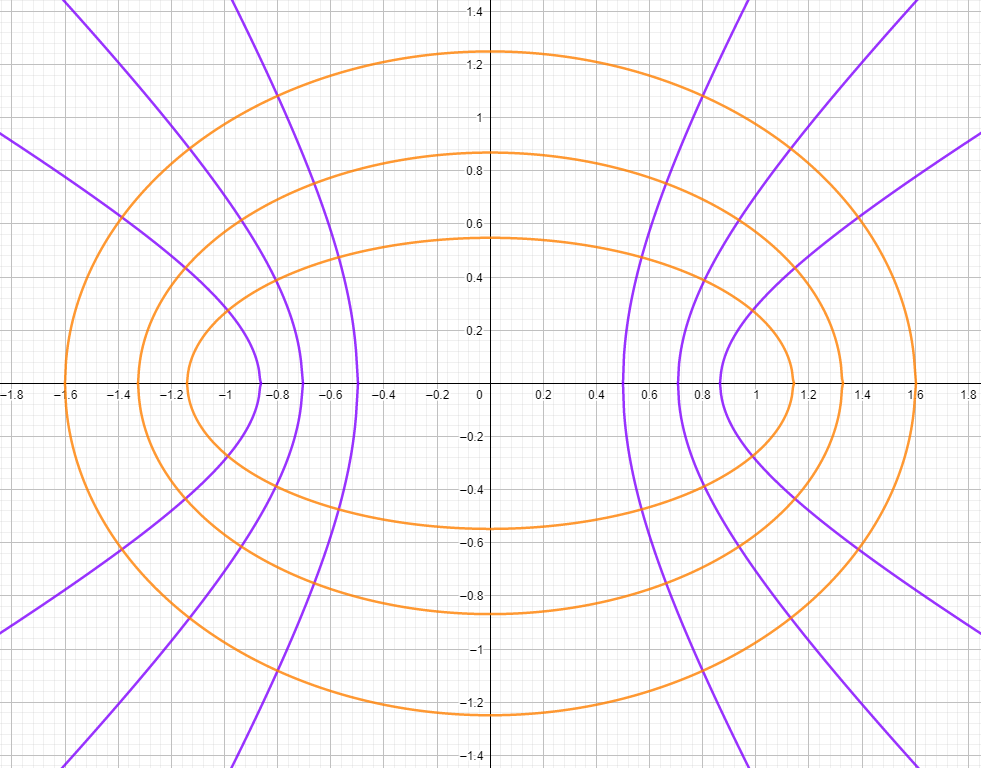
\includegraphics[width=0.5\textwidth]{C.PNG}
    \caption{The orange lines are $u=\frac{\pi}{6}$, $u=\frac{\pi}{4}$, $u=\frac{\pi}{3}$}the purple lines are $v=\frac{\pi}{6}$, $v=\frac{\pi}{4}$, $v=\frac{\pi}{3}$
    \label{fig:C}
\end{figure}

The unit vectors $\VE_u$ and $\VE_v$ are perpendicular to the lines, and pointing right at $x>0$ and pointing left at $x<0$. 

\paragraph{3.10.3}
The unit vectors of orthogonal coordinates are perpendicular to each other, so we have $\VE_i\cdot\VE_j=\delta_{ij}$, and $\VE_i\times\VE_j=\VE_k$. Therefore, $(A_1\VE_1+A_2\VE_2+A_3\VE_3)\cdot(B_1\VE_1+B_2\VE_2+B_3\VE_3)=A_1B_1+A_2B_2+A_3B_3$, and \[(A_1\VE_1+A_2\VE_2+A_3\VE_3)\times(B_1\VE_1+B_2\VE_2+B_3\VE_3)=(A_2B_3-A_3B_2)\VE_1+(A_3B_1-A_1B_3)\VE_2+(A_1B_2-A_2B_1)\VE_3\]

\paragraph{3.10.4}
(a) $\VE_1=1\VE_1+0\VE_2+0\VE_3$. Using the divergence formula for curvilinear coordinates, \[\del\cdot\varphi=\frac{1}{h_1h_2h_3}\pdv{(h_2h_3)}{q_1}\]

(b) 
\[
\del\times\VE_1=\frac{1}{h_1h_2h_3}
\begin{vmatrix}
\VE_1h_1&\VE_2h_2&\VE_3h_3\\
\pdv{}{q_1}&\pdv{}{q_2}&\pdv{}{q_3}\\
h_1&0&0
\end{vmatrix}
\]
\[
=\frac{1}{h_1h_2h_3}\left[\VE_2h_2\pdv{h_1}{q_3}-\VE_3h_3\pdv{h_1}{q_2} \right]
\]
\[
=\frac{1}{h_1}\left[\VE_2\frac{1}{h_3}\pdv{h_1}{q_3}-\VE_3\frac{1}{h_2}\pdv{h_1}{q_2} \right]
\]

\paragraph{*3.10.5}
$\VE_i\cdot\VE_i=1=\frac{1}{h_i^2}\pdv{\V{r}}{q_i}\cdot\pdv{\V{r}}{q_i}=\frac{1}{h_i^2}\left((\pdv{x}{q_1})^2+(\pdv{y}{q_1})^2+(\pdv{x}{q_1})^2 \right)$, so $h_i^2=(\pdv{x}{q_i})^2+(\pdv{y}{q_i})^2+(\pdv{x}{q_i})^2$, in agreement with Eq. 3.131.

From $h_i\VE_i=\pdv{\V{r}}{q_i}$, we can get \[\pdv{h_i}{q_j}\VE_i+h_i\pdv{\VE_i}{q_j}=\pdv{(h_i\VE_i)}{q_j}=\pdv{^2\V{r}}{q_j\partial q_i}
=\pdv{^2\V{r}}{q_i\partial q_j}=\pdv{(h_j\VE_j)}{q_i}=\pdv{h_j}{q_i}\VE_j+h_j\pdv{\VE_j}{q_i}
\]
so
\[
h_i\pdv{\VE_i}{q_j}-\pdv{h_j}{q_i}\VE_j=h_j\pdv{\VE_j}{q_i}-\pdv{h_i}{q_j}\VE_i=\V{a}
\]
If $\V{a}=0$, then $\pdv{\VE_i}{q_j}=\frac{1}{h_i}\pdv{h_j}{q_i}\VE_j$ can be proved. However, I don't know how to prove it. (I know $\V{a}\cdot\VE_i=\V{a}\cdot\VE_j=0$, and also by taking $\V{a}\cdot\V{a}$, it is equivalent to prove $\pdv{\VE_i}{q_j}\cdot\pdv{\VE_j}{q_i}=0$, however, I can't find a proof for this either)

From $\VE_i\cdot\VE_j=0$, we have $\pdv{\VE_i}{q_i}\cdot\VE_j+\VE_i\cdot\pdv{\VE_j}{q_i}=0$, so we have \[\pdv{\VE_i}{q_i}\cdot\VE_j=-\VE_i\cdot\pdv{\VE_j}{q_i}=-\VE_i\cdot\VE_i\frac{1}{h_j}\pdv{h_i}{q_j}=-\frac{1}{h_j}\pdv{h_i}{q_j}\]
Also, $\pdv{\VE_i}{q_i}\cdot\VE_j=\frac{1}{2}\pdv{(\VE_i\cdot\VE_i)}{q_i}=0$, so 
\[
\pdv{\VE_i}{q_i}=\sum_{j\neq i}\VE_j(\pdv{\VE_i}{q_i}\cdot\VE_j)=-\sum_{j\neq i}\VE_j\frac{1}{h_j}\pdv{h_i}{q_j}
\]

\paragraph{3.10.6}
$\V{r}=\rho\cos\varphi\VE_x+\rho\sin\varphi\VE_y+z\VE_z$     
\medskip

$\pdv{\V{r}}{\rho}=\cos\varphi\VE_x+\sin\varphi\VE_y=h_\rho\VE_\rho$, so $h_\rho=1$ and $\VE_\rho=\cos\varphi\VE_x+\sin\varphi\VE_y$

$\pdv{\V{r}}{\varphi}=-\rho\sin\varphi\VE_x+\rho\cos\varphi\VE_y=h_\varphi\VE_\varphi$, so $h_\varphi=\rho$ and $\VE_\varphi=-\sin\varphi\VE_x+\cos\varphi\VE_y$

$\pdv{\V{r}}{z}=\VE_z=h_z\VE_z$, so $h_z=1$ and $\VE_z=\VE_z$

\paragraph{3.10.7}
From Exercise 3.10.6,

$\cos\varphi\VE_\rho-\sin\varphi\VE_\varphi=(\cos^2\varphi+\sin^2\varphi)\VE_x=\VE_x$, so $\VE_x=\cos\varphi\VE_\rho-\sin\varphi\VE_\varphi$

$\sin\varphi\VE_\rho+\cos\varphi\VE_\varphi=(\sin^2\varphi+\cos^2\varphi)\VE_y=\VE_y$, so $\VE_y=\sin\varphi\VE_\rho+\cos\varphi\VE_\varphi$

$\VE_z=\VE_z$

\paragraph{3.10.8}
From exercise 3.10.6,
$\pdv{\VE_\rho}{\varphi}=-\VE_x\sin\varphi+\VE_y\cos\varphi=\VE_\varphi$, and $\pdv{\VE_\varphi}{\varphi}=-\VE_x\cos\varphi-\VE_y\sin\varphi=-\VE_\rho$. All the other derivatives vanish because $\VE_\rho$ and $\VE_\varphi$ are functions of $\varphi$ only, and $\VE_z$ is a constant vector.

\paragraph{3.10.9}
From exercise 3.10.8, $\pdv{\VE_\rho}{\varphi}=\VE_\varphi$ and $\pdv{\VE_\varphi}{\varphi}=-\VE_\rho$, so 
\[
\del\cdot\V{V}=(\VE_\rho\pdv{}{\rho}+\VE_\varphi\frac{1}{\rho}\pdv{}{\varphi}+\VE_z\pdv{}{z})\cdot(\VE_\rho V_\rho+\VE_\varphi V_\varphi+\VE_z V_z)
\]
\[
=\VE_\rho\cdot(\VE_\rho\pdv{V_\rho}{\rho}+\VE_\varphi\pdv{V_\rho}{\rho}+\VE_z\pdv{V_z}{\rho})
+\frac{1}{\rho}\VE_\varphi\cdot(\VE_\varphi V_\rho+\VE_\rho\pdv{V_\rho}{\varphi}-\VE_\rho V_\varphi+\VE_\varphi\pdv{V_\varphi}{\varphi}+\VE_z\pdv{V_z}{\varphi})+\VE_z\cdot(\VE_z\pdv{V_z}{z})
\]
\[
=\pdv{V_\rho}{\rho}+\frac{V_\rho}{\rho}+\frac{1}{\rho}\pdv{V_\varphi}{\varphi}+\pdv{V_z}{z}
\]
\[
=\frac{1}{\rho}\pdv{(\rho V_\rho)}{\rho}+\frac{1}{\rho}\pdv{V_\varphi}{\varphi}+\pdv{V_z}{z}
\]

\paragraph{3.10.10}
(a) From exercise 3.10.6, $\VE_\rho\rho+\VE_z z=\VE_x\rho\cos\varphi+\VE_y\rho\sin\varphi+\VE_z z=\VE_x x+\VE_y y+\VE_z z=\V{r}$

(b) \[\del\cdot\V{r}=\frac{1}{\rho}\pdv{}{\rho}(\rho^2)+\pdv{V_z}{z}=2+1=3\] 
\[
\del\times\V{r}=\frac{1}{\rho}
\begin{vmatrix}
\VE_\rho&\VE_\varphi\rho&\VE_z\\
\pdv{}{\rho}&\pdv{}{\varphi}&\pdv{}{z}\\
\rho&0&z
\end{vmatrix}=0
\]

\paragraph{3.10.11}
(a) A point $P=(\rho\cos\varphi,\rho\sin\varphi,z)$ after reflection would be $P'=(-\rho\cos\varphi,-\rho\sin\varphi,-z)=(\rho\cos(\varphi\pm\pi),\rho\sin(\varphi\pm\pi),-z)$, so it corresponds to the transformation 
\[
\rho\rightarrow\rho,\quad\varphi\rightarrow\varphi\pm\pi,\quad z\rightarrow-z
\]

(b) 
\[
\VE_\rho'=\VE_x\cos(\varphi\pm\pi)+\VE_y\sin(\varphi\pm\pi)=-\VE_x\cos\varphi-\VE_y\sin\varphi=-\VE_\rho
\]
\[
\VE_\varphi'=-\VE_x\sin(\varphi\pm\pi)+\VE_y\cos(\varphi\pm\pi)=\VE_x\sin\varphi-\VE_y\cos\varphi=-\VE_\varphi
\]
\[
\VE_z'=\VE_z
\]

\paragraph{3.10.12}
(a) 
\[
\V{v}=\boldsymbol{\omega}\times\V{r}=(\omega\VE_z)\times(\rho\VE_\varphi+z\VE_z)=\omega\rho\VE_\varphi
\]

(b)
\[
\del\times\V{v}=\frac{1}{\rho}
\begin{vmatrix}
\VE_\rho&\VE_\varphi\rho&\VE_z\\
\pdv{}{\rho}&\pdv{}{\varphi}&\pdv{}{z}\\
0&\omega\rho^2&0
\end{vmatrix}=
\frac{1}{\rho}(2\omega\rho)\VE_z=2\boldsymbol{\omega}
\]

\paragraph{3.10.13}
\[
\frac{d\VE_\rho}{dt}=-\VE_x\dot{\varphi}\sin\varphi+\VE_y\dot{\varphi}\cos\varphi=\VE_\varphi\dot{\varphi}
\]
\[
\frac{d\VE_\varphi}{dt}=-\VE_x\dot{\varphi}\cos\varphi-\VE_y\dot{\varphi}\sin\varphi=-\VE_\rho\dot{\varphi}
\]
\[
\frac{d\VE_z}{dt}=0
\]
\[
\V{r}=\VE_\rho\rho+\VE_z z
\]
\[
\V{v}=\dot{\V{r}}=\VE_\varphi\dot{\varphi}\rho+\VE_\rho\dot{\rho}+\VE_z\dot{z}\]
\[
=\VE_\rho\dot{\rho}+\VE_\varphi\rho\dot{\varphi}+\VE_z\dot{z}
\]
\[
\V{a}=\dot{\V{v}}=\VE_\varphi\dot{\varphi}\dot{\rho}+\VE_\rho\Ddot{\rho}-\VE_\rho\dot{\varphi}\rho\dot{\varphi}+\VE_\rho(\dot{\rho}\dot{\varphi}+\rho\Ddot{\varphi})+\VE_z\Ddot{z}
\]
\[
=\VE_\rho(\Ddot{\rho}-\rho\dot{\varphi
}^2)+\VE_\varphi(\rho\Ddot{\varphi}+2\dot{\rho}\dot{\varphi})+\VE_z\Ddot{z}
\]

\paragraph{3.10.14}
\[
\del\times\V{v}=\frac{1}{\rho}
\begin{vmatrix}
\VE_\rho&\VE_\varphi\rho&\VE_z\\
\pdv{}{\rho}&\pdv{}{\varphi}&\pdv{}{z}\\
V_\rho(\rho,\varphi)&\rho V_\varphi(\rho,\varphi)&0
\end{vmatrix}
=\frac{1}{\rho}\left[\VE_z\left(\pdv{(\rho V_\varphi)}{\rho}-\pdv{V_\rho}{\varphi}\right) \right]
\]

\paragraph{3.10.15}
\[
\V{B}=\del\times\V{A}=\frac{1}{\rho}
\begin{vmatrix}
\VE_\rho&\VE_\varphi\rho&\VE_z\\
\pdv{}{\rho}&\pdv{}{\varphi}&\pdv{}{z}\\
0&0&\frac{\mu I}{2\pi}\ln(\frac{1}{\rho})
\end{vmatrix}
=\frac{1}{\rho}\left[-\VE_\varphi\rho\frac{\mu I}{2\pi}\rho\frac{-1}{\rho^2} \right]=\VE_\varphi\frac{\mu I}{2\pi\rho}
\]

\paragraph{3.10.16}
(a) From exercise 3.10.7, we have
\[
\V{F}=-(\VE_\rho\cos\varphi-\VE_\varphi\sin\varphi)\frac{\rho\sin\varphi}{\rho^2}+(\VE_\rho\sin\varphi+\VE_\varphi\cos\varphi)\frac{\rho\cos\varphi}{\rho^2}=\VE_\rho\frac{1}{\rho}
\]

(b) 
\[
\del\times\V{F}=\frac{1}{\rho}
\begin{vmatrix}
\VE_\rho&\VE_\varphi\rho&\VE_z\\
\pdv{}{\rho}&\pdv{}{\varphi}&\pdv{}{z}\\
0&\rho\frac{1}{\rho}&0
\end{vmatrix}
=0
\]

(c)
\[
\oint(\VE_\varphi\frac{1}{\rho})\cdot(\VE_\rho d\rho+\VE_\varphi\rho d\varphi+\VE_z dz)=\oint d\varphi=2\pi
\]

(d) The range of $\varphi$ of cylindrical coordinates is $0\leq\varphi<2\pi$, so $\int_0^{2\pi}d\varphi$ is not defined.

\paragraph{3.10.17}
\[
(\V{B}\cdot\del)\V{B}=B_\varphi\frac{1}{\rho}\pdv{}{\varphi}(\VE_\varphi B_\varphi(\rho))=\frac{B_\varphi}{\rho}[-\VE_\rho B_\varphi+0]=-\VE_\rho\frac{B_\varphi^2}{\rho}
\]

\paragraph{3.10.18}
\[
\pdv{\V{r}}{r}=\VE_x\sin\theta\cos\varphi+\VE_y\sin\theta\sin\varphi+\VE_z\cos\theta=h_r\VE_r\]
so
\[h_r=1,\quad \VE_r=\VE_x\sin\theta\cos\varphi+\VE_y\sin\theta\sin\varphi+\VE_z\cos\theta
\]
\[
\pdv{\V{r}}{\theta}=\VE_xr\cos\theta\cos\varphi+\VE_y r\cos\theta\sin\varphi-\VE_z r\sin\theta=h_\theta\VE_\theta\]
so
\[h_\theta=r,\quad \VE_\theta=\VE_x\cos\theta\cos\varphi+\VE_y\cos\theta\sin\varphi-\VE_z\sin\theta
\]
\[
\pdv{\V{r}}{\varphi}=-\VE_x r\sin\theta\sin\varphi+\VE_y r\sin\theta\cos\varphi=h_\varphi\VE_\varphi
\]
so
\[
h_\varphi=r\sin\theta,\quad\VE_\varphi=-\VE_x\sin\varphi+\VE_y\cos\varphi
\]

\paragraph{3.10.19}
\begin{equation}
    \VE_r=\VE_x\sin\theta\cos\varphi+\VE_y\sin\theta\sin\varphi+\VE_z\cos\theta
\end{equation}
\begin{equation}
    \VE_\theta=\VE_x\cos\theta\cos\varphi+\VE_y\cos\theta\sin\varphi-\VE_z\sin\theta
\end{equation}
\begin{equation}
    \VE_\varphi=-\VE_x\sin\varphi+\VE_y\cos\varphi
\end{equation}
$\cos\theta\times(1)-\sin\theta\times(2)$, we get 
\[
\VE_z=\VE_r\cos\theta-\VE_\theta\sin\theta
\]
$\sin\theta\times(1)+\cos\theta\times(2)$, we get 
\begin{equation}
    \VE_r\sin\theta+\VE_\theta\cos\theta=\VE_x\cos\varphi+\VE_y\sin\varphi
\end{equation}
$\cos\varphi\times(4)-\sin\varphi\times(3)$, we get
\[
\VE_x=\VE_r\sin\theta\cos\varphi+\VE_\theta\cos\theta\cos\varphi-\VE_\varphi\sin\varphi
\]
$\cos\varphi\times(3)+\sin\varphi\times(4)$, we get
\[
\VE_y=\VE_r\sin\theta\sin\varphi+\VE_\theta\cos\theta\sin\varphi+\VE_\varphi\cos\varphi
\]

\paragraph{3.10.20}
(a) The point $\V{r}=(0,0,0)$ is related to $\V{r'}=(0,\theta,\varphi)$ for any $0\leq\theta\leq\pi$ and $0\leq\varphi<2\pi$. If $\V{r'}=\M{B}\V{r}$, then $\V{r}=(0,0,0)$ can only be related to $\V{r'}=(0,0,0)$, a contradiction, so the matrix $\M{B}$ cannot exist.\\
(If $x,y,z\neq0$, then simply 
\[\M{B}=
\begin{pmatrix}
\frac{r}{x}&0&0\\
0&\frac{\theta}{y}&0\\
0&0&\frac{\varphi}{z}
\end{pmatrix}
\]
satisfies the condition.)

(b)
From exercise 3.10.19,
\[
\V{V}=\VE_xV_x+\VE_yV_y+\VE_zV_z
\]
\[
=(\VE_r\sin\theta\cos\varphi+\VE_\theta\cos\theta\cos\varphi-\VE_\varphi\sin\varphi)V_x
\]
\[+(\VE_r\sin\theta\sin\varphi+\VE_\theta\cos\theta\sin\varphi+\VE_\varphi\cos\varphi)V_y\]
\[+(\VE_r\cos\theta-\VE_\theta\sin\theta)V_z
\]
\[
=\VE_rV_r+\VE_\theta V_\theta+\VE_\varphi V_\varphi
\]
which is
\[
\begin{pmatrix}
V_r\\V_\theta\\V_\varphi
\end{pmatrix}=
\begin{pmatrix}
\sin\theta\cos\varphi&\sin\theta\sin\varphi&\cos\theta\\
\cos\theta\cos\varphi&\cos\theta\sin\varphi&-\sin\theta\\
-\sin\varphi&\cos\varphi&0
\end{pmatrix}
\begin{pmatrix}
V_x\\V_y\\V_z
\end{pmatrix}
\]
Let the matrix be $\M{M}$, and let its transpose be $\V{M}^T$, then it can be verified that $\M{M}\M{M}^T=\boldsymbol{1}$, so it is orthogonal.

\paragraph{3.10.21}
(Let $\varphi$ of spherical coordinate be $\phi$, and $\varphi$ of cylindrical coordinate remain the same.)
The relations between the two coordinates are $\rho=r\sin\theta$, $\varphi=\phi$, $z=r\cos\theta$.
\[
\VE_r=\pdv{\V{r}}{r}=\pdv{\V{r}}{\rho}\pdv{\rho}{r}+\pdv{\V{r}}{\varphi}\pdv{\varphi}{r}+\pdv{\V{r}}{z}\pdv{z}{r}
=\VE_\rho\sin\theta+\VE_\varphi\rho\cdot0+\VE_z\cos\theta
\]
\[
=\VE_\rho\sin\theta+\VE_z\cos\theta
\]
\[
\VE_\theta=\frac{1}{r}\pdv{\V{r}}{\theta}=\frac{1}{r}(\pdv{\V{r}}{\rho}\pdv{\rho}{\theta}+\pdv{\V{r}}{\varphi}\pdv{\varphi}{\theta}+\pdv{\V{r}}{z}\pdv{z}{\theta})=
\frac{1}{r}\VE_\rho r\cos\theta+\frac{1}{r}\VE_\varphi\rho\cdot0+\frac{1}{r}\VE_z(-r\sin\theta)
\]
\[
=\VE_\rho\cos\theta-\VE_z\sin\theta
\]
\[
\VE_\phi=\frac{1}{r\sin\theta}\pdv{\V{r}}{\phi}=\frac{1}{r\sin\theta}(\pdv{\V{r}}{\rho}\pdv{\rho}{\phi}+\pdv{\V{\phi}}{\varphi}\pdv{\varphi}{\phi}+\pdv{\V{r}}{z}\pdv{z}{\phi})=
\frac{1}{r\sin\theta}\VE_\varphi\rho\cdot1
\]
\[
=\VE_\varphi
\]
so
\[
\V{V}=V_r\VE_r+V_\theta\VE_\theta+V_\phi\VE_\phi
\]
\[
=V_r(\VE_\rho\sin\theta+\VE_z\cos\theta)+V_\theta(\VE_\rho\cos\theta-\VE_z\sin\theta)+V_\phi\VE_\varphi
\]
\[
=V_\rho\VE_\rho+V_\varphi\VE_\varphi+V_z\VE_z
\]
which is 
\[
\begin{pmatrix}
V_\rho\\V_\varphi\\V_z
\end{pmatrix}=
\begin{pmatrix}
\sin\theta&\cos\theta&0\\
0&0&1\\
\cos\theta&-\sin\theta&0
\end{pmatrix}
\begin{pmatrix}
V_r\\V_\theta\\V_\phi
\end{pmatrix}
\]
Let the matrix be $\M{M}$. Note that it is orthogonal, so the inverse transformation is 
\[
\M{M}^{-1}=\M{M}^T=
\begin{pmatrix}
\sin\theta&0&\cos\theta\\
\cos\theta&0&-\sin\theta\\
0&1&0
\end{pmatrix}
\]

\paragraph{3.10.22}
(a) 
\begin{align*}
    \pdv{\VE_r}{r}&=0 &
    \pdv{\VE_r}{\theta}&=\VE_\theta&
    \pdv{\VE_r}{\varphi}&=\VE_\varphi\sin\theta\\
    \pdv{\VE_\theta}{r}&=0 &
    \pdv{\VE_\theta}{\theta}&=-\VE_r&
    \pdv{\VE_\theta}{\varphi}&=\VE_\varphi\cos\theta\\
    \pdv{\VE_\varphi}{r}&=0 &
    \pdv{\VE_\varphi}{\theta}&=0&
    \pdv{\VE_\varphi}{\varphi}&=-\VE_r\sin\theta-\VE_\theta\cos\theta \\
\end{align*}

(b)
\[
\del\cdot\del\psi=(\VE_r\pdv{}{r}+\VE_\theta\frac{1}{r}\pdv{}{\theta}+\VE_\varphi\frac{1}{r\sin\theta}\pdv{}{\varphi})\cdot(\VE_r\pdv{\psi}{r}+\VE_\theta\frac{1}{r}\pdv{\psi}{\theta}+\VE_\varphi\frac{1}{r\sin\theta}\pdv{\psi}{\varphi})
\]
\[
=\VE_r\cdot\left(\VE_r\pdv{^2\psi}{r^2}+\VE_\theta(\cdots)+\VE_\varphi(\cdots) \right)
+\frac{1}{r}\VE_\theta\cdot\left(\VE_\theta\pdv{\psi}{r}+\VE_\theta\frac{1}{r}\pdv{^2\psi}{\theta^2}+\VE_r(\cdots)+\VE_\varphi(\cdots) \right)
\]
\[
+\frac{1}{r\sin\theta}\VE_\varphi\cdot\left(\VE_\varphi\sin\theta\pdv{\psi}{r}+\VE_\varphi\cos\theta\frac{1}{r}\pdv{\psi}{\theta}+\VE_\varphi\frac{1}{r\sin\theta}\pdv{^2\psi}{\varphi^2}+\VE_r(\cdots)+\VE_\theta(\cdots) \right)
\]
\[
=\frac{2}{r}\pdv{\psi}{r}+\pdv{^2\psi}{r^2}+\frac{\cos\theta}{r^2\sin\theta}\pdv{\psi}{\theta}+\frac{1}{r^2}\pdv{^2\psi}{\theta^2}+\frac{1}{r^2\sin^2\theta}\pdv{^2\psi}{\varphi^2}
\]
\[
=\frac{1}{r^2\sin\theta}\left[\sin\theta\pdv{}{r}(r^2\pdv{\psi}{r})+\pdv{}{\theta}(\sin\theta\pdv{\psi}{\theta})+\frac{1}{\sin\theta}\pdv{^2\psi}{\varphi^2} \right]
\]

\paragraph{3.10.23}
(a) $\boldsymbol{\omega}=\VE_z\omega=\VE_r\omega\cos\theta-\VE_\theta\omega\sin\theta$, so
\[
\V{v}=\boldsymbol{\omega}\times\V{r}=(\VE_r\omega\cos\theta-\VE_\theta\omega\sin\theta)\times(\VE_r r)=\VE_\varphi\omega r \sin\theta
\]

(b)
\[
\del\times\V{v}=\frac{1}{r^2\sin\theta}
\begin{vmatrix}
\VE_r&\VE_\theta r&\VE_\varphi r\sin\theta\\
\pdv{}{r}&\pdv{}{\theta}&\pdv{}{\varphi}\\
0&0&\omega r^2\sin^2\theta
\end{vmatrix}\]
\[=\frac{1}{r^2\sin\theta}(\VE_r2\omega r^2\sin\theta\cos\theta-\VE_\theta2\omega r^2\sin^2\theta)\]
\[=2\VE_r\omega\cos\theta-2\VE_\theta\omega\sin\theta=2\boldsymbol{\omega}
\]

\paragraph{3.10.24}
\[
\del\times\V{V}=\frac{1}{r^2\sin\theta}
\begin{vmatrix}
\VE_r&\VE_\theta r&\VE_\varphi r\sin\theta\\
\pdv{}{r}&\pdv{}{\theta}&\pdv{}{\varphi}\\
0&V_\theta&V_\varphi
\end{vmatrix}
\]
\[
=\frac{1}{r^2\sin\theta}\left[\VE_r(\pdv{V_\varphi}{\theta}-\pdv{V_\theta}{\varphi})-\VE_\theta r(\pdv{V_\varphi}{r})+\VE_\varphi r\sin\theta(\pdv{V_\theta}{r}) \right]
\]
has no tangential components, so $\pdv{V_\varphi}{r}=\pdv{V_\theta}{r}=0$. That is, the tangential components of $\V{V}$ have no radial dependence.

\paragraph{3.10.25}
(a) A point $P=(r\sin\theta\cos\varphi,r\sin\theta\sin\varphi,r\cos\theta)$ after reflection would become\\ $P'=(-r\sin\theta\cos\varphi,-r\sin\theta\sin\varphi,-r\cos\theta)=(r\sin(\pi-\theta)\cos(\varphi\pm\pi),r\sin(\pi-\theta)\sin(\varphi\pm\pi),r\cos(\pi-\theta))$, so it corresponds to the transformation 
\[
r\rightarrow r,\quad\theta\rightarrow\pi-\theta,\quad \varphi\rightarrow\varphi\pm\pi
\]

(b) 

\[\VE_r'=\VE_x\sin(\pi-\theta)\cos(\varphi\pm\pi)+\VE_y\sin(\pi-\theta)\sin(\varphi\pm\pi)+\VE_z\cos(\pi-\theta)=-\VE_r
\]
\[ \VE_\theta=\VE_x\cos(\pi-\theta)\cos(\varphi\pm\pi)+\VE_y\cos(\pi-\theta)\sin(\varphi\pm\pi)-\VE_z\sin(\pi-\theta)=\VE_\theta
\]
\[
\VE_\varphi=-\VE_x\sin(\varphi\pm\pi)+\VE_y\cos(\varphi\pm\pi)=-\VE_\varphi
\]

\paragraph{3.10.26}
(a)
\[
(\V{A}\cdot\del)\V{r}=(A_x\pdv{}{x}+A_y\pdv{}{y}+A_z\pdv{}{z})(x\VE_x+y\VE_y+z\VE_z)\]
\[=A_x\VE_x+A_y\VE_y+A_z\VE_z=\V{A}
\]

(b) 
From exercise 3.10.22
\[
(\V{A}\cdot\del)\V{r}=(A_r\pdv{}{r}+A_\theta\frac{1}{r}\pdv{}{\theta}+A_\varphi\frac{1}{r\sin\theta}\pdv{}{\varphi})(r\VE_r)=A_r\VE_r+A_\theta\frac{1}{r}r\VE_\theta+A_\varphi\frac{1}{r\sin\theta}r\sin\theta\VE_\varphi\]
\[=A_r\VE_r+A_\theta\VE_\theta+A_\varphi\VE_\varphi=\V{A}
\]

\paragraph{3.10.27}
From exercise 3.10.22
\[
\frac{d\VE_r}{dt}=\pdv{\VE_r}{r}\pdv{r}{t}+\pdv{\VE_r}{\theta}\pdv{\theta}{t}+\pdv{\VE_r}{\varphi}\pdv{\varphi}{t}=\VE_\theta\dot{\theta}+\VE_\varphi\sin\theta\dot{\varphi}
\]
\[
\frac{d\VE_\theta}{dt}=\pdv{\VE_\theta}{r}\pdv{r}{t}+\pdv{\VE_\theta}{\theta}\pdv{\theta}{t}+\pdv{\VE_\theta}{\varphi}\pdv{\varphi}{t}=-\VE_r\dot{\theta}+\VE_\varphi\cos\theta\dot{\varphi}
\]
\[
\frac{d\VE_\varphi}{dt}=\pdv{\VE_\varphi}{r}\pdv{r}{t}+\pdv{\VE_\varphi}{\theta}\pdv{\theta}{t}+\pdv{\VE_\varphi}{\varphi}\pdv{\varphi}{t}=-\VE_r\sin\theta\dot{\varphi}-\VE_\theta\cos\theta\dot{\varphi}
\]
\[
\V{r}=\VE_r r
\]
so
\[
\V{v}=\dot{\V{r}}=\VE_\theta\dot{\theta}r+\VE_\varphi\sin\theta\dot{\varphi}r+\VE_r\dot{r}
\]
\[
=\VE_r\dot{r}+\VE_\theta r\dot{\theta}+\VE_\varphi r\sin\theta\dot{\varphi}
\]
\[
\V{a}=\dot{\V{v}}=\VE_\theta\dot{r}\dot{\theta}+\VE_\varphi\dot{r}\sin\theta\dot{\varphi}+\VE_r\Ddot{r}-\VE_r r{\dot{\theta}}^2+\VE_\varphi r\cos\theta\dot{\theta}\dot{\varphi}+\VE_\theta\dot{r}\dot{\theta}+\VE_\theta r\Ddot{\theta}\]
\[-\VE_r r\sin^2\theta{\dot{\varphi}}^2-\VE_\theta r\sin\theta\cos\theta{\dot{\varphi}}^2+\VE_\varphi\dot{r}\sin\theta\dot{\varphi}+\VE_\varphi r\cos\theta\dot{\theta}\dot{\varphi}+\VE_\varphi r\sin\theta\Ddot{\varphi}
\]
\[
=\VE_r(\Ddot{r}-r{\dot{\theta}}^2-r\sin^2\theta{\dot{\varphi}}^2)+\VE_\theta(r\Ddot{\theta}+2\dot{r}\dot{\theta}-r\sin\theta\cos\theta{\dot{\varphi}}^2)+\VE_\varphi(r\sin\theta\Ddot{\varphi}+2\dot{r}\sin\theta\dot{\varphi}+2r\cos\theta\dot{\theta}\dot{\varphi})
\]

\paragraph{3.10.28}
\[
\del=\VE_x\pdv{}{x}+\VE_y\pdv{}{y}+\VE_z\pdv{}{z}
\]
\[
=\VE_r\pdv{}{r}+\VE_\theta\frac{1}{r}\pdv{}{\theta}+\VE_\varphi\frac{1}{r\sin\theta}\pdv{}{\varphi}
\]
\[
=(\VE_x\sin\theta\cos\varphi+\VE_y\sin\theta\sin\varphi+\VE_z\cos\theta)\pdv{}{r}
\]
\[
+(\VE_x\cos\theta\cos\varphi+\VE_y\cos\theta\sin\varphi-\VE_z\sin\theta)\frac{1}{r}\pdv{}{\theta}
\]
\[
+(-\VE_x\sin\varphi+\VE_y\cos\varphi)\frac{1}{r\sin\theta}\pdv{}{\varphi}
\]
\[
=\VE_x(\sin\theta\cos\varphi\pdv{}{r}+\cos\theta\cos\varphi\frac{1}{r}\pdv{}{\theta}-\frac{\sin\varphi}{r\sin\theta}\pdv{}{\varphi})
\]
\[
+\VE_y(\sin\theta\sin\varphi\pdv{}{r}+\cos\theta\sin\varphi\frac{1}{r}\pdv{}{\theta}+\frac{\cos\varphi}{r\sin\theta}\pdv{}{\varphi})
\]
\[
+\VE_z(\cos\theta\pdv{}{r}-\sin\theta\frac{1}{r}\pdv{}{\theta})
\]
equating the $x,y,z$ components, we get
\[
\pdv{}{x}=\sin\theta\cos\varphi\pdv{}{r}+\cos\theta\cos\varphi\frac{1}{r}\pdv{}{\theta}-\frac{\sin\varphi}{r\sin\theta}\pdv{}{\varphi}
\]
\[
\pdv{}{y}=\sin\theta\sin\varphi\pdv{}{r}+\cos\theta\sin\varphi\frac{1}{r}\pdv{}{\theta}+\frac{\cos\varphi}{r\sin\theta}\pdv{}{\varphi}
\]
\[
\pdv{}{z}=\cos\theta\pdv{}{r}-\sin\theta\frac{1}{r}\pdv{}{\theta}
\]

\paragraph{3.10.29}
$x=r\sin\theta\cos\varphi$, $y=r\sin\theta\sin\varphi$. Using results from exercise 3.10.28, we can have
\[
x\pdv{}{y}-y\pdv{}{x}=r\sin\theta\cos\varphi(\sin\theta\sin\varphi\pdv{}{r}+\cos\theta\sin\varphi\frac{1}{r}\pdv{}{\theta}+\frac{\cos\varphi}{r\sin\theta}\pdv{}{\varphi})\]
\[-r\sin\theta\sin\varphi(\sin\theta\cos\varphi\pdv{}{r}+\cos\theta\cos\varphi\frac{1}{r}\pdv{}{\theta}-\frac{\sin\varphi}{r\sin\theta}\pdv{}{\varphi})
=\pdv{}{\varphi}
\]
so 
\[-i\left(x\pdv{}{y}-y\pdv{}{x}\right)=-i\pdv{}{\varphi}\]

\paragraph{3.10.30}
\[
\V{L}=-i(\V{r}\times\del)=-i(\VE_r r)\times(\VE_r\pdv{}{r}+\VE_\theta\frac{1}{r}\pdv{}{\theta}+\VE_\varphi\frac{1}{r\sin\theta}\pdv{}{\varphi})
\]
\[
=\VE_\theta i\frac{1}{\sin\theta}\pdv{}{\varphi}-\VE_\varphi i\pdv{}{\theta}
\]
\[
=(\VE_x\cos\theta\cos\varphi+\VE_y\cos\theta\sin\varphi-\VE_z\sin\theta)i\frac{1}{\sin\theta}\pdv{}{\varphi}+(\VE_x\sin\varphi-\VE_y\cos\varphi)i\pdv{}{\theta}
\]
\[
=\VE_x(i\sin\varphi\pdv{}{\theta}+i\cot\theta\cos\varphi\pdv{}{\varphi})+\VE_y(-i\cos\varphi\pdv{}{\theta}+i\cot\theta\sin\varphi\pdv{}{\varphi})+\VE_z(-i\pdv{}{\varphi})
\]
so
\[
L_x+iL_y=i\sin\varphi\pdv{}{\theta}+i\cot\theta\cos\varphi\pdv{}{\varphi}+\cos\varphi\pdv{}{\theta}-\cot\theta\sin\varphi\pdv{}{\varphi}
\]
\[
=(\cos\varphi+i\sin\varphi)(\pdv{}{\theta}+i\cot\theta\pdv{}{\varphi})=e^{i\varphi}(\pdv{}{\theta}+i\cot\theta\pdv{}{\varphi})
\]
\[
L_x-iL_y=i\sin\varphi\pdv{}{\theta}+i\cot\theta\cos\varphi\pdv{}{\varphi}-\cos\varphi\pdv{}{\theta}+\cot\theta\sin\varphi\pdv{}{\varphi}
\]
\[
=(-\cos\varphi+i\sin\varphi)(\pdv{}{\theta}-i\cot\theta\pdv{}{\varphi})=-e^{-i\varphi}(\pdv{}{\theta}-i\cot\theta\pdv{}{\varphi})
\]

\paragraph{3.10.31}
From exercise 3.10.30
\[
\V{L}=\VE_xL_x+\VE_yL_y+\VE_zL_z\]
\[=\VE_x(i\sin\varphi\pdv{}{\theta}+i\cot\theta\cos\varphi\pdv{}{\varphi})+\VE_y(-i\cos\varphi\pdv{}{\theta}+i\cot\theta\sin\varphi\pdv{}{\varphi})+\VE_z(-i\pdv{}{\varphi})
\]
so 
\[
\V{L}\times\V{L}=\VE_x(L_yL_z-L_zL_y)+\VE_y(L_zL_x-L_zL_z)+\VE_z(L_xL_y-L_yL_x)
\]
\[
=\VE_x(-\sin\varphi\pdv{}{\theta}-\cot\theta\cos\varphi\pdv{}{\varphi})+\VE_y(\cos\varphi\pdv{}{\theta}-\cot\theta\sin\varphi\pdv{}{\varphi})+\VE_z(\pdv{}{\varphi})
\]
\[
=\VE_xiL_x+\VE_yiL_y+\VE_ziL_z=i\V{L}
\]

\paragraph{3.10.32}
(a)(b) It is the first half of exercise 3.10.30.

(c) The author suggest to do it in Cartesian coordinate, but I think it's easier to do in spherical coordinate, with the help of results from 3.10.22(a).
\[
{\V{L}}^2=\V{L}\cdot\V{L}=-(\VE_\theta\frac{1}{\sin\theta}\pdv{}{\varphi}-\VE_\varphi\pdv{}{\theta})\cdot(\VE_\theta\frac{1}{\sin\theta}\pdv{}{\varphi}-\VE_\varphi\pdv{}{\theta})
\]
\[
=-\left[\VE_\theta\frac{1}{\sin\theta}\cdot\pdv{}{\varphi}(\VE_\theta\frac{1}{\sin\theta}\pdv{}{\varphi}) +\VE_\varphi\cdot\pdv{}{\theta}(\VE_\varphi\pdv{}{\theta})-\VE_\theta\frac{1}{\sin\theta}\cdot\pdv{}{\varphi}(\VE_\varphi\pdv{}{\theta})-\VE_\varphi\cdot\pdv{}{\theta}(\VE_\theta\frac{1}{\sin\theta}\pdv{}{\varphi})\right]
\]
\[
=-\left[\frac{1}{\sin^2\theta}\pdv{^2}{\varphi^2}+\pdv{^2}{\theta^2}+\frac{\cos\theta}{\sin\theta}\pdv{}{\theta} \right]
\]
\[
=-\frac{1}{\sin\theta}\pdv{}{\theta}(\sin\theta\pdv{}{\theta})-\frac{1}{\sin^2\theta}\pdv{^2}{\varphi^2}
\]
\[
=-r^2\del^2+\pdv{}{r}\left(r^2\pdv{}{r} \right)
\]
(We use Eq. 3.158 in the last equality.)

\paragraph{3.10.33}
(a) 
\[
\VE_r\pdv{}{r}-i\frac{\V{r}\times\V{L}}{r^2}=\VE_r\pdv{}{r}-\frac{\V{r}\times(\V{r}\times\del)}{r^2}=\VE_r\pdv{}{r}-\frac{\V{r}(\V{r}\cdot\del)-(\V{r}\cdot\V{r})\del}{r^2}=\VE_r\pdv{}{r}-\frac{\VE_r r(r\pdv{}{r})-r^2\del}{r^2}=\del
\]

(b) (\textit{There is probably a mistake:} $\del(1+r\pdv{}{r})$ \textit{should be} $\del+\del(r\pdv{}{r})$)
\smallskip

$r\pdv{}{r}=\V{r}\cdot\del$ in the spherical coordinate, so the left side of the equation is $\V{r}\del^2-\del-\del(\V{r}\cdot\del)$.
\[
\left[\V{r}\del^2-\del-\del(\V{r}\cdot\del) \right]_x=x(\pdv{^2}{x^2}+\pdv{^2}{y^2}+\pdv{^2}{z^2})-\pdv{}{x}-\pdv{}{x}(x\pdv{}{x}+y\pdv{}{y}+z\pdv{}{z})
\]
\[
=-2\pdv{}{x}+x\pdv{^2}{y^2}+x\pdv{^2}{z^2}-y\pdv{^2}{x\partial y}-z\pdv{^2}{x\partial z}
\]
\[
\left[i\del\times\V{L} \right]_x=\left[\del\times(\V{r}\times\del) \right]_x=\pdv{}{y}(x\pdv{}{y}-y\pdv{}{x})-\pdv{}{z}(z\pdv{}{x}-x\pdv{}{z})
\]
\[
=-2\pdv{}{x}+x\pdv{^2}{y^2}+x\pdv{^2}{z^2}-y\pdv{^2}{x\partial y}-z\pdv{^2}{x\partial z}
\]
So the $x$-components of two side of the equation are equal. It can be verified that so are the $y$- and $z$-components. Therefore,
\[
\V{r}\del^2-\del-\del(\V{r}\cdot\del)=i\del\times\V{L}
\]

\paragraph{3.10.34}
\[
\frac{1}{r^2}\frac{d}{dr}\left[r^2\frac{d\psi}{dr} \right]=\frac{1}{r^2}(2r\frac{d\psi}{dr}+r^2\frac{d^2\psi}{dr^2})=\frac{d^2\psi}{dr^2}+\frac{2}{r}\frac{d\psi}{dr}
\]
\[
\frac{1}{r}\frac{d^2}{dr^2}\left[r\psi\right]=\frac{1}{r}\frac{d}{dr}(\psi+r\frac{d\psi}{dr})=\frac{1}{r}(\frac{d\psi}{dr}+\frac{d\psi}{dr}+r\frac{d^2\psi}{dr^2})=\frac{d^2\psi}{dr^2}+\frac{2}{r}\frac{d\psi}{dr}
\]
so all the three form are equaivalant.

\paragraph{3.10.35}
(a)
\[
\del\times\V{F}=\frac{1}{r^2\sin\theta}
\begin{vmatrix}
\VE_r&\VE_\theta r&\VE_\varphi r\sin\theta\\
\pdv{}{r}&\pdv{}{\theta}&\pdv{}{\varphi}\\
\frac{2P\cos\theta}{r^3}&\frac{P}{r^2}\sin\theta&0\\
\end{vmatrix}
=\frac{1}{r^2\sin\theta}\left(\VE_\varphi r\sin\theta(-2\frac{P}{r^3}\sin\theta+\frac{2P\sin\theta}{r^3}) \right)=0
\]

(b) $r=1$ and $\theta=\frac{\pi}{2}$, so $\V{F}=\VE_\theta P$ and $d\V{r}=\VE_r dr+\VE_\varphi d\varphi$. 
\[
\oint\V{F}\cdot d\V{r}=(\VE_\theta P)\cdot(\VE_r dr+\VE_\varphi d\varphi)=0
\]
We cannot assert whether $\V{F}$ is conservative or not unless we evaluate every integral over closed loop.

(c) $\int_a^b\V{F}\cdot d\V{r}=\psi(a)-\psi(b)$. Take the path $(r,\theta,\varphi)\rightarrow(\infty,\theta,\varphi)$, and define the potential at infinity $\psi(\infty)$ to be zero. Then we have
\[
\psi(\V{r})=\psi(\V{r})-\psi(\infty)=\int_r^\infty\frac{2P\cos\theta}{r^3}dr=-\frac{P\cos\theta}{r^2}\Big|_r^\infty=\frac{P\cos\theta}{r^2}
\]

\paragraph{3.10.36}
(a)
\[
\del\times\V{A}=\frac{1}{r^2\sin\theta}
\begin{vmatrix}
\VE_r&\VE_\theta r&\VE_\varphi r\sin\theta\\
\pdv{}{r}&\pdv{}{\theta}&\pdv{}{\varphi}\\
0&0&-\cos\theta
\end{vmatrix}
=\frac{1}{r^2\sin\theta}(\VE_r\sin\theta)=\frac{\VE_r}{r^2}
\]

(b) $r=\sqrt{x^2+y^2+z^2}$, $\theta=\cos^{-1}\frac{z}{r}$, $\varphi=\tan^{-1}\frac{y}{x}$, $\VE_\varphi=-\VE_x\sin\varphi+\VE_y\cos\varphi$. So
\[
\V{A}=-(-\VE_x\frac{y}{\sqrt{x^2+y^2}}+\VE_y\frac{x}{\sqrt{x^2+y^2}})\frac{z}{\sqrt{x^2+y^2}}\frac{1}{r}=\VE_x\frac{yz}{r(x^2+y^2)}-\VE_y\frac{xz}{r(x^2+y^2)}
\]

(c)
\[
\del\times\V{A}=\frac{1}{r^2\sin\theta}
\begin{vmatrix}
\VE_r&\VE_\theta r&\VE_\varphi r\sin\theta\\
\pdv{}{r}&\pdv{}{\theta}&\pdv{}{\varphi}\\
0&-\varphi\sin\theta&0
\end{vmatrix}
=\frac{1}{r^2\sin\theta}(\VE_r\sin\theta)=\frac{\VE_r}{r^2}
\]

\paragraph{3.10.37}
$\V{r}=\VE_r r$, so from exercise 3.10.22 we have $\pdv{\V{r}}{r}=\VE_r$, $\pdv{\V{r}}{\theta}=\VE_\theta r$, $\pdv{\V{r}}{\varphi}=\VE_\varphi r\sin\theta$. So
\[
\V{E}=-\del\psi=-\left[\VE_r\pdv{}{r}(\frac{\V{P}\cdot\V{r}}{4\pi\varepsilon_0r^3})+\VE_\theta\frac{1}{r}\pdv{}{\theta}(\frac{\V{P}\cdot\V{r}}{4\pi\varepsilon_0r^3})+\VE_\varphi\frac{1}{r\sin\theta}\pdv{}{\varphi}(\frac{\V{P}\cdot\V{r}}{4\pi\varepsilon_0r^3}) \right]
\]
\[
=-\VE_r\left(\frac{1}{4\pi\varepsilon_0r^3}\V{P}\cdot\pdv{\V{r}}{r}+\frac{\V{P}\cdot\V{r}}{4\pi\varepsilon_0}\pdv{}{r}(\frac{1}{r^3})\right)-\VE_\theta\frac{1}{r}\frac{1}{4\pi\varepsilon_0r^3}\V{P}\cdot\pdv{\V{r}}{\theta}-\VE_\varphi\frac{1}{r\sin\theta}\frac{1}{4\pi\varepsilon_0r^3}\V{P}\cdot\pdv{\V{r}}{\varphi}
\]
\[
=-\VE_r(-2)\frac{P_r}{4\pi\varepsilon_0r^3}-\VE_\theta\frac{P_\theta}{4\pi\varepsilon_0r^3}-\VE_\varphi\frac{P_\varphi}{4\pi\varepsilon_0r^3}
\]
\[
=\frac{1}{4\pi\varepsilon_0r^3}(3\VE_rP_r-\VE_rP_r-\VE_\theta P_\theta-\VE_\varphi P_\varphi)
\]
\[
=\frac{3\hat{\V{r}}(\V{P}\cdot\hat{\V{r}})}{4\pi\varepsilon_0r^3}
\]
where $\hat{\V{r}}=\VE_r$ is the unit vector in the $\V{r}$ direction.







\end{document}
